\documentclass[12pt]{article}

\usepackage{amsmath}    % need for subequations
\usepackage{graphicx}   % need for figures
\usepackage{verbatim}   % useful for program listings
\usepackage{color}      % use if color is used in text
\usepackage{subfigure}  % use for side-by-side figures
\usepackage{hyperref}   % use for hypertext links, including those to external documents and URLs
\usepackage{latexsym}
\usepackage{amsfonts}
\usepackage{graphicx} 
\usepackage{amsthm}
\usepackage{listings}


% don't need the following. simply use defaults
\setlength{\baselineskip}{16.0pt}    % 16 pt usual spacing between lines

\setlength{\parskip}{3pt plus 2pt}
\setlength{\parindent}{20pt}
\setlength{\oddsidemargin}{0.5cm}
\setlength{\evensidemargin}{0.5cm}
\setlength{\marginparsep}{0.75cm}
\setlength{\marginparwidth}{2.5cm}
\setlength{\marginparpush}{1.0cm}
\setlength{\textwidth}{150mm}

\newtheorem{theorem}{Theorem}[section]
\newtheorem{corollary}{Corollary}[theorem]
\newtheorem{lemma}[theorem]{Lemma}
% above is the preamble

\begin{document}

\begin{titlepage}


\begin{center}


% Oberer Teil der Titelseite:

\includegraphics[width=0.35\textwidth]{./lmu_siegel}\\[1.0cm]    

\textsc{\LARGE Ludwig-Maximilians-Universit\"at M\"unchen}\\[1.5cm]

\textsc{\Large Master's Thesis}\\[0.5cm]


% Title
\newcommand{\HRule}{\rule{\linewidth}{0.5mm}}
\HRule \\[0.4cm]
{ \huge \bfseries The Vectorial Deffuant Model}\\[0.2cm]

\HRule \\[1.5cm]

% Author and supervisor
\begin{minipage}{0.4\textwidth}
\begin{flushleft} \large
\emph{Author:}\\
Alexander\\ \textsc{Mendelsohn}
\end{flushleft}
\end{minipage}
\hfill
\begin{minipage}{0.4\textwidth}
\begin{flushright} \large
\emph{Supervisor:} \\
Prof. Dr. Markus \textsc{Heydenreich}
\end{flushright}
\end{minipage}

\vfill

% Unterer Teil der Seite
{\large \today}

\end{center}

\end{titlepage}

\newpage
\thispagestyle{empty}
\mbox{}
\clearpage

\tableofcontents
\thispagestyle{empty}
\clearpage

\newpage
\thispagestyle{empty}
\mbox{}
\clearpage
\setcounter{page}{1}

\section{Introduction}

In recent years there has been a growing interest in agent-based models as a means to understanding the long-term behaviour of complex social-systems in social sciences. Cultural dissemination and opinion dynamics are modelled as a process where traits are propagated from person to person in a larger social network. The model itself is characterised by heuristic rules determining the outcomes of  interaction between two agents and a spacial structure, modelling the social network as a graph, that encodes the pairs of agents that may interact due to social contact. The central objective when studying such models is to deduce macroscopic behaviour, i.e. the behaviour of the society as a whole, which arises from microscopic rules, i.e. rules for interaction between individuals. Within the field of mathematics agent-based models are called interacting particle systems. The models are of course the same in both fields, but their methodologies of research differ. The study of  agent-based models is concerned with numerical simulation whereas interacting particle systems is concerned  with rigorous analytical results. Rigorous mathematical research in this field started only a few years ago with the work of Nicolas Lanchier and with the notable exception of the voter model there is an apparent lack of analytical results for these models. Particularly for models such as the vectorial Deffuant model which has many more absorbing states than the voter model analytical results are quintessential because simulations of the finite system can freeze in a number of states which are not symptomatic of the long-term behaviour of their infinite counterparts. 

The vectorial Deffuant model was proposed by Guillaume Deffuant et. al. as a model for opinion dynamics. It models the dynamics of a set of non-independent opinions and is an extension of the voter model. The heuristic microscopic rules make two agreeable assumptions on the interaction between individuals: homophily, the tendency of individuals to interact with individuals who are similar, and social influence, the tendency of individuals to become more similar through interaction. Homophily is modelled with an interaction threshold. Individuals are characterised by a vector of $F$ coordinates each of which assumes one of two different states ("for" or "against"). Individuals  who differ in two many opinions, more than a given threshold, cease to interact with one another. When two agents do not breach the threshold, their interaction entails choosing a differing feature at random and one of the agents imitating the other with respect to this feature. The interaction threshold is what makes opinions non-independent and sets the vectorial Deffuant model apart from the voter model. Note that the voter model also models social influence but cannot model homophily since individuals either completely agree or disagree with one another. 
The vectorial Deffuant Model is very similar to Robert Axelrod's  stochastic model for cultural dissemination. In the Axelrod model individuals are characterised by a vector of $F$ coordinates each of which assumes one of $q$ different states. This vector is supposed to represent someone's entire culture, i.e. "[...] the set of individual attributes that are subject to social influence."\cite[p. 204]{Axelrod} Interaction rules are here also based on the assumptions of homophily and social influence. Homophily is modelled by making pairs of neighbours interact at a rate equal to the fraction of features they have in common. 
The vectorial Deffuant model and the Axelrod model are two very similar models which were proposed to model two \textit{not} entirely different concepts. In fact, one might say culture and opinion a very much intertwined. Comparing these two models we are confronted with an immediate short-coming. Even though they are mathematically interesting and incredibly intricate their epistemological significance is subverted by the vagueness of the actual concept they aim to model. 
The main objective here is to find analytical results for the vectorial Deffuant model and a modification of it, which will be introduced as the dissociating vectorial Deffuant model. However, we first introduce a more specific interpretation of the model. 

"If such a thing as an advanced study of human behaviour exists, linguists may claim to hold that position -- perhaps for no other reason than its ability to state precisely the issues being argued. [...] The question of 'One phoneme vs. Two' has a more precise meaning than similar questions that might be raised concerning, e.g. two statuses or roles, two memories, or two personalities." \cite[p. 267]{Labov}
We here use the vectorial Deffuant model to model language change --  cultural dissemination concerning only a subset of culture. The social phenomenon we identify with the vectorial Deffuant model is that of the change of pronunciations in dialects, known as vowel shifts. A particular vowel sound, a phoneme, such as the /ohr/ sound found in \textit{born, forth, fort, horns, source ...} can undergo a pronunciation shift $/ohr/ \rightarrow /uweh/$, as it has in recent decades in the northern cities of the USA. Hence, each agent is characterised by a vector of $F$ coordinates representing $F$ lexemes (words) containing the same phoneme (sound). The values assumed for each coordinate, 0 and 1, then represent the traditional and the new pronunciation. When agents interact they imitate their neighbour's pronunciation of a particular word and new pronunciation standards can be achieved across the entire social network.

Changes in social or cultural factors may encourage a community of speakers and listeners to favour a new variant of pronunciation over a standard one. And many sound changes have been recorded empirically. However, there is still much dispute about how the sound change takes place. 
There are two, not entirely opposing, theories of sound change: (1) The Neogrammarian stance claims that the basic unit of change is the sound, the phoneme, and that all words containing the sound are effected equally. This concept is also called regular sound change and is still supported by William Labov. (2) Lexical Diffusion denotes the idea that the basic unit of sound change is the word itself. "Phonological change propagates itself gradually across the lexicon, from morpheme to morpheme."\cite[p. 255]{Chen}
We are here concerned with the implementation (how) and not the actuation (why) of such a phonological process occurs. As stated by Chen and Wang: "Two concepts are fundamental here: the temporal and the lexical dimensions of a phonological process. Oddly enough, one of the the most neglected aspects of historical linguistics, which professes to be a study of language evolving across time, is the time element itself. Of course much discussion has been devoted to the relative chronology of phonological processes, but this concerns the external relation between rules in terms of time sequence; the internal time dimension has not received equal attention until fairly recent times." \cite[256]{Chen}
To study how a sound change can be consolidated in a population through interaction between its individuals, we consider the hypothetical case that a phonological unit has been entirely destabilized. All individuals initially pronounce each lexeme in one of two possible manners at random. The objective of the model is then to study how and if a standard of pronunciation is achieved through propagation on a social network.
Such a destabilized state can occur within a speech community through immigration, cultural influences and the random mutations of individuals' phoneme realization. We are here not concerned with this highly contextual aspect of the process of language evolution. This thesis is only concerned with how a speech community mitigates a heterogeneous phoneme use.  

To interpret the model correctly one should keep in mind what assumptions are made. Homophily and social influence are, as stated, the central assumptions but implicitly we also assume that there is no central authority and that agents are adaptive rather than rational. Language is of course standardised, canonised and influenced by persons of authority. The present model, however, is concerned with the process of social influence before the actions of such authorities. Agents are simply modelled to adapt to their environment, to speak more like their neighbours speak. Agents do not make choices based on strategic or cost-benefit analyses. If we consider that even the idea that language will always develop towards greater efficiency and comprehensibility has been rejected empirically, the assumptions made here are reasonable and minimal.
The model assumes a position somewhere between the Neogrammarian and lexical diffusionist dichotomy. In the initial configuration of the system the phoneme is assumed to be destabilized, independent of the actual lexeme. And interaction between two agents results in a change of pronunciation of a particular lexeme only.
The \textit{dissociating} vectorial Deffuant model which we will introduce makes a further assumption: the tendency of speakers to seek regularity. There are two extremal configurations an individual can assume, all lexemes follow the traditional pronunciation or all lexemes follow the new pronunciation -- all other configurations lie in between these two states. The dissociating vectorial Deffuant model assumes that if two agents who both lean towards the same extremal configuration interact, then the outcome of their interaction will favour the agent who is closest to the extremal state. 
The spatial structure, the integer lattice, does not make any assumptions about the geographic distribution of agents. The integer lattice should be considered a generalized social network. More complex social networks could be constructed, however, in the absence of universally credible networks the integer lattice is a perfectly good starting point. What is of interest here are the global dynamics induced by a person-to-person propagation. And the integer lattice is a connected network where each individual is only directly connected to a few others. Additionally, the integer lattice allows us to analyse the system analytically.

Agent-based models have to date found very little application in linguistic research. "Language dynamics is an emerging field that focuses on all processes related to emergence, change, evolution, interactions and extinction of languages. [...] Models for language dynamics and evolution can be roughly divided in two main categories: socio-biological and sociocultural approaches."\cite[27]{Castellano} The most influential microscopic model of language dynamics was introduced by Schulze and Stauffer in 2005 and their approach is socio-biological. "The similarity of the evolution of human languages to biological evolution of species is utilized to study [...] the rise and fall of languages [...]" \cite[86]{Schulze} in a model for the competition of languages. 
Their attribute space, a vector of $F$ components each assuming one of two possible states, is the same as ours but the model is entirely different. They attempt to model the development of all human language throughout the scope man's existence. Their model does not include a spatial structure and the evolution rules are inspired by biological predator-prey models:
In the Stauffer/Schulz model agents give birth to offspring which speak their parents' language and random mutation of their parents' language. Agents die at a rate determined by the overall population size and a carrying capacity constant, which includes factors like limited space and resources. Additionally, agents switch languages at a rate determined by the respective language dominance. 
They have managed to replicate empirical data -- the number of languages follows a log-normal distribution in time. However, there are some rather strong assumptions made to "fit the data". Languages of small sizes shrink and go extinct and do not show resilience as they do in reality. Language diversity begins to diminish after the entire population has reached a growth plateau induced by the so-called carrying capacity -- humanity has to date not experienced any such growth plateau. And new languages are assumed to be started by individuals who then begin to propagate the language through offspring. 
Our approach is sociocultural. The vectorial Deffuant model is a model of interaction that does incorporate death and procreation. Dissemination within an existing population is studied. There is of course the possibility to make interaction rules depend on the proportional dominance of a configuration in the larger system. This would model social-influence in a population where agents are aware of global trends. As mentioned above, however, we choose not to incorporate any form of central authority because it could obscure the mechanism of dissemination which we are interested in. 

\textbf{Structure of Thesis:} The microscopic rules of the vec. Deff. model are convergent -- agents become become more alike -- but the system as a whole can show polarizing limiting behaviours. In Section 2 the mathematical model is introduced, tools needed later are introduced and three classes of limiting behaviour are introduced: (1) \textit{clustering} -- complete consensus is achieved in the limit; (2) \textit{fixation} -- a limiting (random) configuration is achieved eventually; (3) \textit{fluctuation} - the configuration of each agent changes at arbitrarily large times. 
In Section 3 we prove fluctuation and clustering results for the 2-Feature vec. Deff. model (2 features, threshold 1).
In Section 4 fixation of the 2-Feature dissociating vec. Deff. model is proven on $\mathbb{Z}^d$, $d\geq 1$.
In Section 5 we deduce a sufficient condition for fixation on $\mathbb{Z}$ and prove fixation for a number of parameter combinations.
Lastly, Section 6 is devoted analysing simulations of the vec. Deff. model on a torus and making closing remarks on the significance of such simulations for research on language change.



\section{The Model}


\subsection{Model Description}

The vectorial Deffuant model was introduced by \cite{Deffuant et al.} as a model for opinion dynamics which incorporates homophily and social influence.
It is an interacting particle system, i.e. a Feller process whose state at time $t \in \mathbb{R}_{\geq 0}$ is a function that maps the vertex set $V$ of a graph $G=(V,E)$ into a set of attributes
\begin{equation}
\eta_t : V \longrightarrow \Gamma := \text{ attribute space } 
\end{equation}

\begin{figure}[h]
  \centering
  \begin{minipage}[h]{0.4\textwidth}
    
\includegraphics[width=\textwidth]{c:/users/alexander/graphics/vDF4T2init.PNG}
    \caption{Initial configuration of vec. Deff. model: F=4, $\theta=2$, V = $100\times 100$ torus.}
  \end{minipage}
  \hfill
  \begin{minipage}[h]{0.4\textwidth}
    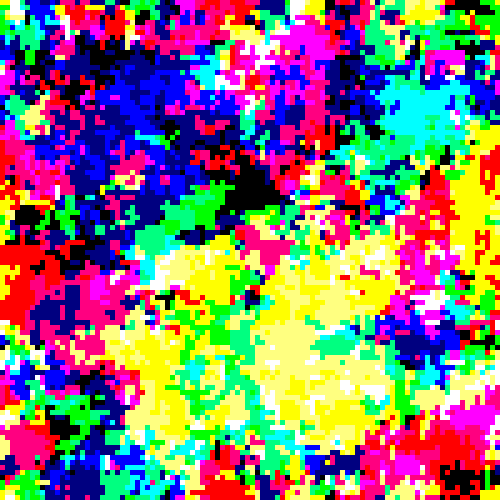
\includegraphics[width=\textwidth]{c:/users/alexander/graphics/vDF4T2_10mil.PNG}
    \caption{Simulation after 10 million successful interactions (changes in configuration).}
  \end{minipage}
\end{figure}

The attribute space $\Gamma$ consists of $F\in \mathbb{N}$ ordered features where each feature can either be configured to $0$ or $1$. Hence, the attribute space is the hypercube equipped with the Hamming distance: 
\begin{equation}
\Gamma := \{0,1\}^{F} \text{ and }
H: \Gamma^2 \rightarrow \mathbb{N}, \: H(u,v):= \vert \{ i: u_{i} \neq v_{i} \} \vert.
\end{equation}
$\Gamma^V$ is then called \textit{state space} of the system. The system depends on a confidence threshold which will be called $\theta$, where $\theta \in \{0,1,...,F\}$. To describe the dynamics of the system we introduce the set
\begin{equation}
\Omega(x,y,\eta) := \{u \in \Gamma: H(u,\eta(y)) = H(\eta(x),\eta(y))-1\}
\end{equation}
for each $x,y \in V$ and each configuration $\eta$ (i.e. $\eta \in \Gamma^V$). The model can then formally be described as a Feller process with the probability generator
\begin{equation}
\begin{split}
Lf(\eta) = & \sum_{x} {\vert \{y:y \sim x\} \vert}^{-1} \sum_{y \sim x} {\vert \Omega(x,y,\eta) \vert}^{-1} \\ 
& \sum_{u \in \Omega(x,y,\eta)} 1 _{\{ 1 \leq H(\eta(x),\eta(y)) \leq \theta \}} 
[ f(\eta_{x,u})-f(\eta)],
\end{split} 
\end{equation}
where $x\sim y$ denotes that $x$ and $y$ are nearest neighbour (connected by an edge on the graph) vertices and $\eta_{x,u}$ is the configuration obtained from the configuration $\eta$ by setting the configuration at $x$ equal to the configuration $u$ and leaving all the other sites unchanged. And $f$ is a continuous real-valued function with $\vert\vert\vert f \vert\vert\vert := \sum_{x,u}sup_{\eta}\vert f(\eta_{x,u})-f(\eta)\vert < \infty$. \\
As a model for cultural dynamics, the vectorial Deffuant model describes a number of people or agents -- the vertices of the graph $V$ -- who are connected via edges to other agents. Each agent, at an exponentially distributed time, randomly selects one of the agents she is connected with, the two agents compare their features and if no more than $\theta$ of their features differ in configuration they interact: they randomly select one of the features in the attribute space which differ and set their configurations of this feature equal. Which agent has to change his configuration, is chosen randomly with equal probability. \\
\newline
 
We will also be considering the vectorial Deffuant model with a certain bias which may be interpreted as a drift towards the extremal states $(0,0,...,0)$ and \\ 
$(1,1,...,1)$, simply denoted $0$ and $1$. We will call this model the \textit{dissociating vec. Deff. Model}. Here, we consider that an agent's configuration can be closer to one of the extremal states, in terms of Hamming distance, or is central, i.e. exactly half of her attributes are configured to $1$. When two agents interact whose configurations are both closer to one of the extremal states or one the agents has a central configuration, the result of their interaction is probabilistically in favour of the extremer configuration.  To describe the dynamics of this system for each $x\in V$, $u \in \Gamma$ and $\eta \in \Gamma^V$ we further introduce: 
\begin{equation}
d(u) := \min \{H(0,u),H(1,u)\},
\end{equation}
\begin{equation}
A_{x,u} := \{\eta \in \Gamma^V:d(\eta(x))= H(i,\eta(x))\text{ and }d(u)= H(i, u) \text{ for } i\in \{0,1\} \}
\end{equation}
and
\begin{equation}
K(x,u,\eta) := \kappa 1_{\{d(u) < d(\eta(x))\}\cap\{\eta \in A_{x,u}\} } + 1_{\{d(u) \geq d(\eta(x))\} \cup \{\eta \not\in A_{x,u}\}},
\end{equation}

for $\kappa > 1$. The dissociating vec. Deff. model can be defined as the Feller process with probability generator

\begin{equation}
\begin{split}
Lf(\eta) = & \sum_{x} {\vert \{y:y \sim x\} \vert}^{-1} \sum_{y \sim x} {\vert \Omega(x,y,\eta) \vert}^{-1} \\ 
& \sum_{u \in \Omega(x,y,\eta)} 1 _{\{ 1 \leq H(\eta(x),\eta(y)) \leq \theta \}} 
K(x,u,\eta)[ f(\eta_{x,u})-f(\eta)].
\end{split} 
\end{equation}

Having defined the probability generators, we now define three types of limiting behaviour the standard and the dissociating vec. Deff. model can display.

\subsection{Flux, Fixation and Clustering}

The behaviours which are of central interest when studying such a process are fluctuation, fixation and clustering. The notions were first introduced by \cite{Griffeath89} and are defined as follows:\\
\textbf{Fluctuation} occurs whenever 
\begin{equation}
P(\eta_t(x) \neq \eta_s(x)\text{ for some } t>s ) = 1 \: \forall x\in V \: \forall s>0.
\end{equation} 
\textbf{Fixation} occurs if there exists a configuration $\eta_{\infty}$ such that 
\begin{equation}
P(\eta_t(x) = \eta_{\infty}(x) \text{ eventually in } t) = 1 \: \forall x\in V,
\end{equation}
i.e. the attributes of each individual are only updated a finite number of times, and a coexistence of different configurations persists. \
\textbf{Clustering} occurs if
\begin{equation}
\lim_{t \rightarrow \infty} P(\eta_t(x) = \eta_{t}(y)) = 1 \: \forall x,y\in V,
\end{equation}
i.e. there is a convergence to global consensus. \\
The behaviour of the system not only depends on the graph but it also depends on the number of Features $F$ and the threshold $\theta$. For example $\theta =0$ leads to immediate fixation. Note that fluctuation and fixation are mutually exclusive but clustering either coincides with fluctuation or fixation. \\
In order to derive the limiting behaviour two important tools needed. We introduce these in Section 2.3 and 2.4.

\subsection{Coupling with annihilating random walks}
We define a coupling with a collection of annihilating random walks when the graph is the one-dimensional $\mathbb{Z}$-lattice ($G= \mathbb{Z}$-lattice, $V= \mathbb{Z}$). This is done by visualizing the edge between two nearest neighbours $x \sim y \in V$ as a space occupied by particles on $F$ levels. A particle at level $i$ on the edge $e=xy$ represents a disagreement between $x$ and $y$ on the feature $i$. The attribute space is now visualised less as a hypercube but rather as a vertical tuple. To make this rigorous we define 
\begin{equation}
\tilde{\eta_t}: V \times \{1,2,...,F\} \rightarrow \{0,1\} \text{ where } \tilde{\eta_t}(x,i) := \text{ $i^{th}$ coordinate of } \eta_t(x).
\end{equation}
The process corresponding to disagreements is defined by 
$$\xi_t(e,i):= 1_{\{\tilde{\eta_t}(x,i) \neq \tilde{\eta_t}(y,i)\}},$$
where $e=xy$. And we place a particle at level $i$ on edge $e$ if $\xi_t(e,i)= 1$. \\
\begin{figure}[ht]
\centering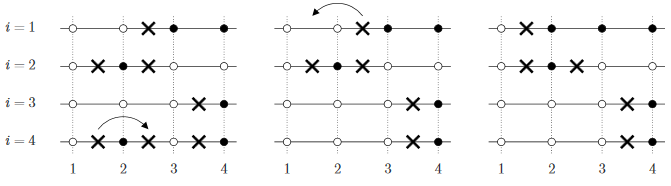
\includegraphics[width=0.7\linewidth]{c:/users/alexander/graphics/annihilatingParticles.PNG}
\caption[width=0.7\linewidth]{\footnotesize{Illustration of the coupling between the vectorial Deffuant model and the system of simple symmetric annihilating random walks. Black and white dots represent the possible configuration on each level while the crosses indicate the position of the particles. The left image represents the agent at site 2 imitating the agent at site 1 w.r.t. feature 4; in the central image 2 imitates 3 w.r.t. feature 1; the right image gives the result of these interactions. \cite{ClustCoex}}}
\end{figure}
The process $\xi$ is key to understanding the dynamics of the model because extinction of particles is equivalent to a clustering of the system. In the standard vec. Deff. model with $G= \mathbb{Z}$-lattice, $\xi_t$ corresponds to a system of F symmetric annihilating random walks which have valuable monotonicity traits.\
For an edge $e=xy$ we define $\zeta_t(e)$ to be the number of particles on the edge at time $t\geq 0$. It holds that $\zeta_t(e)$ is also the Hamming distance between $x$ and $y$ on the attribute space, since
\begin{equation}
\zeta_t(e) 
:= \xi_t(e,1)+\xi_t(e,2)+...+\xi_t(e,F)
= H(\eta_t(x),\eta_t(y)).
\end{equation}
In the case that $G= \mathbb{Z}$-lattice, an  edge will be referred to as a \textbf{blockade} if more than $\theta$ particles are on the edge and as an \textbf{active edge} if at most $\theta$ particles are on the edge. Particles on a blocked edge will be referred as \textit{frozen} and \textit{active} otherwise.
It is important to note that the F systems of annihilating random walks are \textbf{non-independent}. The features which neighbours disagree on are chosen for update uniformly at random. At each edge occupied by $m$ particles, the particles jump at rate equal to
\begin{equation}
r(m) := \left\{\begin{array}{cl} m^{-1}, & \mbox{if } 0<m \leq \theta\\ 0, & \mbox{if}\ \theta < m \leq F. \end{array}\right.
\end{equation}
This coupling will be the key ingredient to proving clustering in Section 3. 

\subsection{The Graphical Representation}

\indent The argumentation throughout will rely strongly on the use of couplings and duality. This section simply defines the percolation structure (graphical representation) from which the coupled system of annihilating random walks and the dual process can be constructed using a standard argument  due to Harris \cite{Harris}. 
The percolation structure consists of a random graph (subset of $G\times \mathbb{R}$) involving independent Poisson processes which give the times at which interactions occur and additional independent Bernoulli random variables and independent uniform random variables to determine the outcome of each interaction.\\
Let $(x,y,i)\in V  \times V \times \{1,2,...,F\}$ where $x \sim y$.
\begin{itemize}
\item We let $(N_{x,y,i}(t):t \geq 0)$ be a collection of rate one Poisson process.
\item We let $T_{x,y,i}(n)$ denote the $n^{th}$ arrival time, i.e. $T_{x,y,i}(n):= \inf\{t:N_{x,y,i}=n\}$.
\item We let $(B_{x,y,i}(n):n \geq 1)$ be a collection of independent Bernoulli random variables with
\begin{equation}
P(B_{x,y,i}(n)=+1)=P(B_{x,y,i}(n)=-1)=1/2.
\end{equation}
\item We let $(U_{x,y,i}(n): n \geq 1)$ be collection of independent Uniform(0,1) random variables.
\end{itemize}
At each time $t:=T_{x,y,i}(n)$ an arrow is drawn from x to y with label $i$, $x\longrightarrow y$ if $B_{x,y,i}(n)=+1$ and from y to x if $B_{x,y,i}(n)=-1$.\
A graphical representation of the dissociating vec. Deff. model can be achieved by simply changing the distribution of the Bernoulli random variables and making them depend on the configuration at x and y at time $t= T_{x,y,i}(n-1)$.\
The arrow $x\longrightarrow y$ is called active iff
\begin{equation}
\xi_{t-}(e,i)= 1 \text{ and } U_{x,y,i}(n) \leq r(\zeta_{t-}(e)),
\end{equation}
where $e=xy$ and $r$ as defined in (14). Now the vectorial Deffuant model and the system of annihilating random walks, in the case $V= \mathbb{Z}$, can be constructed from the graphical representation by assuming that only active arrows have an effect on either system. If there is an active $i$-arrow from x to y at time $t$ then
\begin{itemize}
\item ,at time $t$, the individual at $y$ looks at the individual at $x$ and imitates her opinion for the $i^{th}$ feature -- we set $\tilde{\eta_t}(y,i)=\tilde{\eta}_{t-}(x,i)$ --
\item and the particle at $e$ jumps to the next edge adjacent to $y$.
\end{itemize}
\indent We say there is an active-$i$-path from $(z,s)$ to $(x,t)$, denoted $(z,s) \rightsquigarrow^{i} (x,t)$, whenever there are sequences of times and vertices
$$ s_0 =s<s_1<...<s_{n+1}=t \text{ and } x_0=z, x_1, ...,x_n=x$$
such the following conditions hold:
\begin{itemize}
\item for $j= 1,2,...,n$, there is an active-$i$-arrow $x_{j-1} \longrightarrow x_j$ at time $s_j$, and 
\item for $j= 1,2,...,n$, there is no active-$i$-arrow pointing at $\{x_j\} \times (s_j, s_{j+1})$.
\end{itemize}
And there is a \textit{generalized active path} \footnote{For now, the notion of a generalized active is merely a technicality. It will be used in Section 3 when establishing a sufficient condition for fixation in 1 dimension.} from $(z,s)$ to $(x,t)$, denoted $(z,s) \rightsquigarrow (x,t)$, if 
\begin{itemize}
\item for $j=1,2,...,n$, there is an active arrow $x_{j-1} \longrightarrow x_j$ at time $s_j$.
\end{itemize}
Active $i$-paths establish a form of ancestry. For every space-time point $(x,t)$ there is a unique space-time point $(z,0)$, in the initial configuration, such that both points are connected by an active $i$-path. Hence, $\tilde{\eta_t}(x,i)=\tilde{\eta}_{0}(z,i)$. Generalized active paths can be seen as concatenations of active $i$-paths for possibly different values of $i$.\\
The foundation have been laid and we commence with analytical results in the next section.


\section{2-Feature vectorial Deffuant Model}
We now consider our model with attribute space $\Gamma = {\{0,1\}}^2$ ($F=2$) and threshold\footnote{For $F=2$, $\theta=0$ leads to immediate fixation and $\theta=2$ simply corresponds to two independent voter models.} $\theta=1$ on the $\mathbb{Z}^d$-lattice. We will also assume that the process starts from a product measure with positive type densities.\
The following fluctuation result will be proven in two steps. We first define a coupling between the 2-Feature vec. Deff. model and the voter model. We then prove fluctuation for the voter model in all dimensions, elaborating a proof given by N. Lanchier. The following theorem then follows from a coupling argument. 
Fluctuation of the vec. Deff. model will then be used to prove clustering of the model in one dimension in the last part of this section.

\begin{theorem}
The vectorial Deffuant model with $F=2$ and $\theta=1$ on $\mathbb{Z}^d$ started from a product measure with positive type densities fluctuates for all $d \geq 1$.
\end{theorem}

In order to obtain results on fluctuation we define a coupled process:
\begin{equation}
\rho_t(x) :=  \vert \tilde{\eta}_{t}(x,1)-\tilde{\eta}_{t}(x,2) \vert \text{ for } x \in \mathbb{Z}^d.
\end{equation}
By letting $A_1 := \{(0,1),(1,0)\}$ and $A_0 := \{(1,1),(0,0)\}$, the process $\rho$ can also be obtained by putting $\rho_t(x)= 1_{\{\eta_t(x) \in A_1\}}$, and we can derive the local transition rates of $\rho$:
\begin{equation}
\begin{split}
c_{0 \rightarrow 1}(x,\rho)&= \lim_{h \rightarrow 0}\frac{1}{h}P(\rho_{t+h}=1 \vert \rho_t(x)=0)\\
&=\lim_{h \rightarrow 0}\frac{1}{h} \sum_{i \in A_0}P(\rho_{t+h}=1 \vert \eta_t(x)=i)P(\eta_t(x)=i \vert \rho_t(x)=0) \\
&= \lim_{h \rightarrow 0}\frac{1}{h} \sum_{i \in A_0}\sum_{j \in A_1}P(\eta_{t+h}=j \vert \eta_t(x)=i)P(\eta_t(x)=i \vert \rho_t(x)=0) \\
&= \sum_{i \in A_0}\sum_{j \in A_1}c_{i \rightarrow j}(x,\eta)P(\eta_t(x)=i \vert \rho_t(x)=0) \\
&= \sum_{i \in A_0}\sum_{j \in A_1} \frac{1}{2d} \vert \{ y \sim x: \eta_t(y)=j\} \vert P(\eta_t(x)=i \vert \rho_t(x)=0) \\
&= \sum_{j \in A_1} \frac{1}{2d} \vert \{ y \sim x: \eta_t(y)=j\} \vert \\
&= \frac{1}{2d} \vert \{ y \sim x: \rho_t(y)=1\} \vert.
\end{split}
\end{equation}
Analogously, we obtain that
\begin{equation}
c_{1 \rightarrow 0}(x,\rho)= \frac{1}{2d} \vert \{ y \sim x: \rho_t(y)=0\} \vert.
\end{equation}
Hence, it follows that $\rho$ is the voter model. And a fluctuation of the 2-feature vec. Deff. model is equivalent to fluctuation of the voter model, since for a given $s>0$ we have
\begin{equation}
\begin{split}
&P(\eta_t(x) \neq \eta_s(x)\text{ for some } t>s ) \\
&= P(\tilde{\eta}_{t}(x,1) \neq \tilde{\eta}_{s}(x,1) \text{ and } \tilde{\eta}_{t}(x,2) = \tilde{\eta}_{s}(x,2) \text{ for some } t>s ) \\ &+P(\tilde{\eta}_{t}(x,2) \neq \tilde{\eta}_{s}(x,2) \text{ and } \tilde{\eta}_{t}(x,1) = \tilde{\eta}_{s}(x,1) \text{ for some } t>s ) \\ 
&= P(\rho_t(x) \neq \rho_s(x)\text{ for some } t>s ).
 \end{split}
\end{equation}

Figure 4-7 compare the evolution of the 2-feature vec. Deff. model and the voter model.

\begin{figure}[h]
  \centering
  \begin{minipage}[h]{0.4\textwidth}
    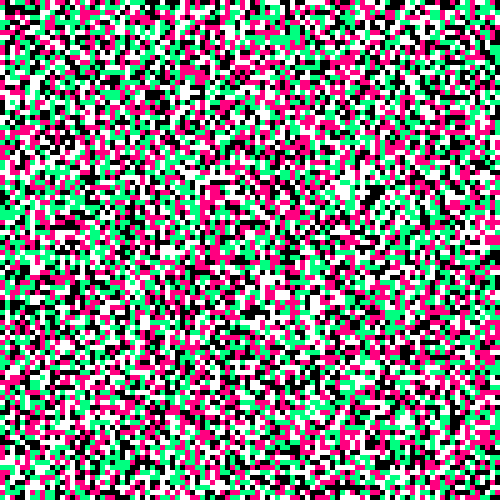
\includegraphics[width=\textwidth]{c:/users/alexander/graphics/vDF2T1init.PNG}
    \caption{Initial configuration: F=2, $\theta=1$, $100\times 100$ torus.}
  \end{minipage}
  \hfill
  \begin{minipage}[h]{0.4\textwidth}
    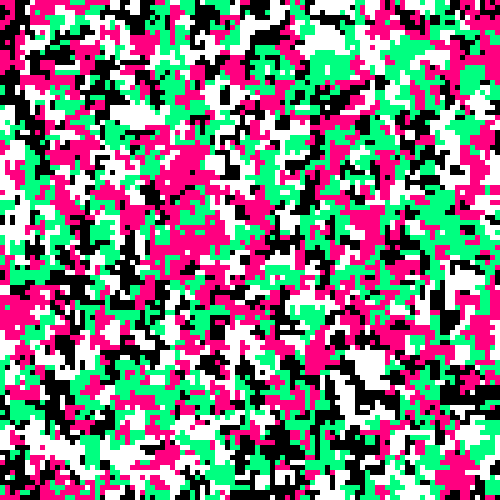
\includegraphics[width=\textwidth]{c:/users/alexander/graphics/vDF2T1.PNG}
    \caption{Simulation after 2 million successful interactions.}
  \end{minipage}
\end{figure}

\begin{figure}[h]
  \centering
  \begin{minipage}[h]{0.4\textwidth}
    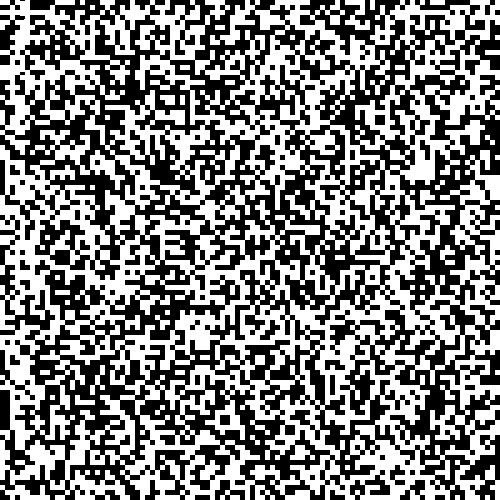
\includegraphics[width=\textwidth]{c:/users/alexander/graphics/voterModelinit.PNG}
    \caption{Initial configuration: voter model, $100\times 100$ torus.}
  \end{minipage}
  \hfill
  \begin{minipage}[h]{0.4\textwidth}
    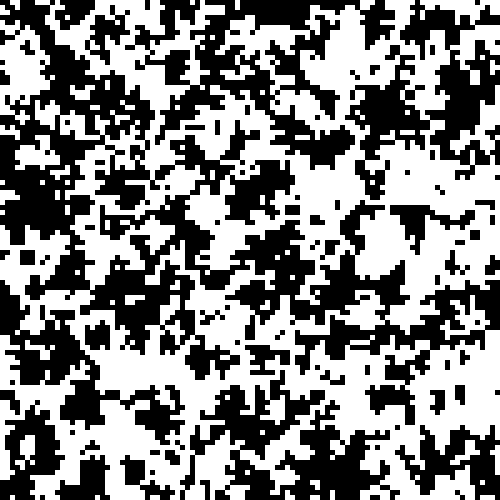
\includegraphics[width=\textwidth]{c:/users/alexander/graphics/voterModel.PNG}
    \caption{Simulation after 1 million successful interactions.}
  \end{minipage}
\end{figure}

We now prove fluctuation for the voter model as stated in the following Lemma.

\begin{lemma}
The voter model fluctuates on $\mathbb{Z}^d$, that is,
\begin{equation}
P(\rho_t(x) \neq \rho_s(x)\text{ for some } t>s ) = 1 \; \forall x\in \mathbb{Z}^d \: \forall s>0.
\end{equation}
\end{lemma}

\begin{proof}
We have assumed that the process starts from a product measure with positive type densities. Hence, $\rho_t$ is the voter model started from a Bernoulli product measure with $B_q(\rho(x)=1)=q \in ]0,1[$. \
The \textit{law of large numbers for occupation time} as proven in \cite{Cox} states that $T^x_t/t \overset{t \rightarrow \infty}{\longrightarrow} q$ almost surely if $d \geq 2$, where $T^x_t= \int_0^t \rho_s(x)ds$ is the \textit{occupation time}. This implies that $\rho$ fluctuates for $d \geq 2$. The case that $d=1$ is somewhat more laborious. \\
\underline{$d=1$:} The proof follows the proof of Lemma 4. in \cite{AxelrodRevised}. \\
For $y \in \mathbb{Z}$ the process 
$$ M_t(y) := \vert \{ z \in \mathbb{Z}: \text{ there is a dual path from } (z,t) \text{ to  }(y,0) \} \vert $$
is a martingale measurable w.r.t. the graphical representation of the voter model with absorbing state $0$. Let $\mathcal{F}_t = \sigma (N_{x,y}(s),B_{x,y}(n); s \leq t, n \leq  N_{x,y}(t), x \sim y)$ for $t\in [0,\infty)$ be a filtration, where $N_{x,y}(s),B_{x,y}(n)$ for $x \sim y \in \mathbb{Z}$ denote the rate 1 independent Poisson processes and the independent Bernoulli random variables from the construction of the graphical representation.  Let $0=\sigma_0< \sigma_1 < \sigma_2 <...$ be the sequence of random transition times of $M_t(y)$, i.e. $\sigma_n := \inf \{s>\sigma_{n-1}: N_{x,y}(s)>N_{x,y}(s-) \text{ for some } x\in M_{\sigma_{n-1}}(y)\}$. Then $\sigma_n- \sigma_{n-1}< \infty$ almost surely for all $n \in \mathbb{N}$ and, since $M_{\sigma_{n-1}}(y)$ consists of at most $n$ sites, at most one Poisson process jumps in the time interval $[\sigma_{n-1},\sigma_{n}]$ almost surely. It then holds for $[s,t]\subseteq [\sigma_{n-1}, \sigma_{n}]$ that

\begin{equation}
\begin{split}
&E[M_{t}(y)-M_{s}(y) \vert \mathcal{F}_{s}] = P(M_{t}(y)-M_{s}(y)= 1\vert \mathcal{F}_{s}) - P(M_{t}(y)-M_{s}(y)= -1\vert \mathcal{F}_{s})\\
&\overset{*}{=} 0. 
\end{split}
\end{equation}

*Since all interactions between two individuals are equally likely to affect the configuration of each individual. Hence, for arbitrary $t>s$ it follows with the tower property that
\begin{equation}
\begin{split}
&E[M_{t}(y)-M_{s}(y) \vert \mathcal{F}_s] \\
&=E[\sum_{n\geq 0}(M_{(\sigma_{n+1}\vee s)\wedge t}(y)-M_{(\sigma_{n}\vee s)\wedge t}(y))\vert\mathcal{F}_s ]\\
&=E[\sum_{n\geq 0}E[M_{(\sigma_{n+1}\vee s)\wedge t}(y)-M_{(\sigma_{n}\vee s)\wedge t}(y)\vert \mathcal{F}_{(\sigma_{n}\vee s)\wedge t}]\vert\mathcal{F}_s ]\\
&=0.
\end{split}
\end{equation}

It follows that $M_t(y)$ is a right-continuous integer-valued martingale with \\ $E[\vert M_t(y)\vert]=E[ M_t(y)]= E[ M_t(y) \vert \mathcal{F}_0]=1$ for all $t>0$.\\
It follows from the martingale convergence theorem that $M_t(y)$ converges to its absorbing state $0$ almost surely. Further, the stopping time $\tau_y = \inf \{ t>0: M_t(y) = 0 \}$ is almost surely finite. \ Let $x \in \mathbb{Z}$ and $s>0$. We define a sequence of increasing stopping times $s_0 = s < s_1 < s_2 < ...$ recursively:
$$ s_{i+1} : = \tau_y(s_i) = \inf \{ t>0: M_t(y) = 0 \} \text{ where } y:= \hat{\rho}_{s_i}^{(x,s_i)}$$
($\hat{\rho}_s^{(A,t)} = \{ z \in \mathbb{Z}: \text{ there is dual path from } (x,t) \text{ to } (z,t-s) \text{ for an } x \in A\}$ denotes the dual process of the voter model -- see Appendix). There is a dual path from $(x, s_{i+1})$ to $(y, s_i)$ for all $i \in \mathbb{N}$, so this stopping time is larger than $s_i$, but almost sure convergence of $M_t(y)$ to zero in finite time implies that time $s_{i+1}$ is almost surely finite. The values $\rho_{s_i}(x)$ are independent for all $i \geq 0$, i.e. determined from the configurations of different sites at time 0. It follows
$$ P(\rho_{s_0}(x) = \rho_{s_1}(x) = ... = \rho_{s_i}(x)) \overset{i \rightarrow \infty}{\longrightarrow} 0. $$
Hence, the system must fluctuate.
\end{proof}

With fluctuation of the 2-feature vec. Deff. model in hand, we are now able to prove clustering in one dimension. We now return to the perspective of annihilating random walks. As mentioned before, extinction of particles is equivalent to clustering of the system. And to prove that all particles go extinct we have to ensure that no particles remain frozen on blocked edges. Fluctuation implies that no edge can remain blocked forever.

\begin{theorem}
The vectorial Deffuant model with $F=2$ and $\theta=1$ on $\mathbb{Z}$ started from a product measure with positive type densities clusters.
\end{theorem}

\begin{proof}
The proof follows a proof for the clustering of the Axelrod Model given in \cite{AxelrodRevised}. \
Consider the continuous time process
$$ u(t) := E(\zeta_t(e)) = P(\zeta_t(e)=1)+2P(\zeta_t(e)=2),$$
where $\zeta_t(e)$ gives the number of particles on edge $e \in E(\mathbb{Z})$, as defined at (13). $u(t)$, the expected number of particles per edge, is independent of the edge $e$ due to translation invariance of the initial configuration and symmetric evolution rules. Because $u(t)$ is determined by a system of symmetric annihilating random walks on $\mathbb{Z}$, it is non-increasing in time. Hence, the limit $\lim_{t \rightarrow \infty} u(t)$ exists almost surely. \\
Let $e=(x)(x+1)$ be an edge with $\zeta_t(e)>0$. Then the edge $e$ is either a blockade or an active edge.
\begin{itemize}
\item If $e$ is a blockade ($\zeta_t(e)=2$), it follows that either $\eta_t(x),\eta_t(x+1) \in A_0$ or $\eta_t(x),\eta_t(x+1) \in A_1$. Which is equivalent to $\rho_t(x)= \rho_t(x+1)$. Since the voter model $\rho$ fluctuates it follows that the blockade is lifted in finite time:
$$ \tau := \inf \{ s>t: \zeta_s(e) \neq 2 \} = \inf \{ s>t: \rho_s(x) \neq \rho_s(x+1) \} < \infty \text{ a.s.}. $$
\item If $e$ is an active edge, it follows from the recurrence of 1 dimensional symmetric random walks that the active particle at $e$ eventually hits another particle and annihilates or forms a blockade. In which case we return to the previous point.
\end{itemize}
It follows, $u(t)$ is strictly decreasing as long as it is positive and $\lim_{t \rightarrow \infty} P (\zeta_t(e) \neq 0)=0 \: \forall e \in E(\mathbb{Z})$. \
For $x,y \in \mathbb{Z}$, $x<y$ we have 
\begin{equation}
\begin{split}
\lim_{t \rightarrow \infty} P (\eta_t(x) \neq \eta_t(y)) & \leq \lim_{t \rightarrow \infty} P (\zeta_t(e) \neq 0 \text{ for some } e) \\
& \leq \lim_{t \rightarrow \infty} \sum_{e \in E(\mathbb{Z})} P (\zeta_t(e) \neq 0) \overset{dom. conv.}{=}0.
\end{split}
\end{equation}
\end{proof}

This proof idea cannot be generalized to higher dimensions because particles representing disagreements follow branching random walks in higher dimensions and do not have monotonicity traits. In the next section, we consider the dissociating vec. Deff. model. Fixation results will follow from a coupling argument similar to the one used for Theorem 3.1..

\section{Fixation of the 2-Feature dissociating vec. Deff. Model}

We now consider the dissociating vec. Deff. model with $F=2$ and $\theta = 1$. First we show that the process $\rho$, as defined in (17), is a biased voter model. We then use results from Bramson and Griffeath \cite{Griffeath81} to prove fixation on $\mathbb{Z}$. \\
For $F=2$ and $\theta=1$ the flip rates of the dissociating vec. Deff. model are given by:
\begin{equation}
\begin{split}
&c_{i \rightarrow j}(x,\eta)=0 \text{ for } i,j \in A_0 \text{ or } i,j \in A_1,\\
&c_{i \rightarrow j}(x,\eta)=\kappa \frac{1}{2d} \vert \{ y \sim x: \eta_t(y)=j\} \vert \text{ for } j \in A_0 \text{ and } i \in A_1,\\
&c_{i \rightarrow j}(x,\eta)=\frac{1}{2d} \vert \{ y \sim x: \eta_t(y)=j\} \vert \text{ for } i \in A_0 \text{ and } j \in A_1,
\end{split}
\end{equation}
where $A_0=\{(0,0),(1,1)\}$, $A_1=\{(1,0),(0,1)\}$ and $\kappa>1$. It follows that the flip rates of process $\rho$ are given by
\begin{equation}
\begin{split}
c_{1 \rightarrow 0}(x,\rho)&= \lim_{h \rightarrow 0}\frac{1}{h}P(\rho_{t+h}=0 \vert \rho_t(x)=1)\\
&=\lim_{h \rightarrow 0}\frac{1}{h} \sum_{i \in A_1}P(\rho_{t+h}=0 \vert \eta_t(x)=i)P(\eta_t(x)=i \vert \rho_t(x)=1) \\
&= \lim_{h \rightarrow 0}\frac{1}{h} \sum_{i \in A_1}\sum_{j \in A_0}P(\eta_{t+h}=j \vert \eta_t(x)=i)P(\eta_t(x)=i \vert \rho_t(x)=1) \\
&= \sum_{i \in A_1}\sum_{j \in A_0}c_{i \rightarrow j}(x,\eta)P(\eta_t(x)=i \vert \rho_t(x)=1) \\
&= \sum_{i \in A_1}\sum_{j \in A_0} \kappa \frac{1}{2d} \vert \{ y \sim x: \eta_t(y)=j\} \vert P(\eta_t(x)=i \vert \rho_t(x)=1) \\
&= \sum_{j \in A_0} \kappa\frac{1}{2d} \vert \{ y \sim x: \eta_t(y)=j\} \vert 
\end{split}
\end{equation}
\begin{equation}\notag
\begin{split}
&= \kappa \frac{1}{2d} \vert \{ y \sim x: \rho_t(y)=0\} \vert.
\end{split}
\end{equation}
Analogously, we obtain
\begin{equation}
c_{0 \rightarrow 1}(x,\rho)= \frac{1}{2d} \vert \{ y \sim x: \rho_t(y)=1\} \vert.
\end{equation}
Hence, it follows that $\rho$ is the biased voter model. 
We are able to apply results for the biased voter model (also called the \textit{Williams-Bjerknes Tumour Growth model}) studied by Bramson and Griffeath in \cite{Griffeath81}. \\
Let $\rho^{B_0}_t := \{x \in \mathbb{Z}^d: \rho_t(x)=0, \rho_0 = 1-1_{\{ B_0 \}}\}$ \\
$= \{ x: \text{there is a path up from }(y,0) \text{ to } (x,t) \text{ for some }y \in B_0\}$ be the process which keeps track of the sites with configuration $0$ started from the initial configuration $\rho_0 = 1-1_{\{ B_0 \}}$ for $B_0 \subseteq \mathbb{Z}^d$. Then $\rho^{0}_t$ is the process started from the configuration with $0$ at the origin and $1$ elsewhere.
And let $\tau^0_{\emptyset}:= \inf\{t>0 : \rho^0_t = \emptyset \}$. The gambler's ruin formula yields that $P(\tau^0_{\emptyset} = \infty)> 0$. If $\tau_n$ denotes the $n^{th}$ time a jump occurs in the process $\rho^{\{0\}}_t$ and $S_n := \vert \rho^{\{0\}}_t \vert $, then $S_n$ is a simple random walk on $\mathbb{N}$ with positive drift $\frac{\kappa-1}{\kappa +1}$ and absorbing state $0$. Hence, the gambler's ruin formula gives that
\begin{equation}
\begin{split}
 &P(\tau^0_{\emptyset} < \infty)= P(S_n = 0 \text{ for some  } n)= \kappa^{-1} < 1 \text{ since, } \kappa >1 \\
 &\Rightarrow P(\tau^0_{\emptyset} = \infty)> 0.
 \end{split}
 \end{equation}
\\
Let $D_R := \{ x \in \mathbb{Z}^d : \Vert x \Vert \leq R \}$ for some $R \geq 1$ be a sphere surrounding the origin ($\Vert\Vert =$ Euklidean norm) and $D_{x,R}= x + D_R$ be a sphere surrounding some $x \in \mathbb{Z}^d$. We quote the main result from Bramson and Griffeath \cite{Griffeath81}. 

\begin{lemma}[\cite{Griffeath81}Theorem 1.]
For $\rho^0_t$ and $\kappa > 1$, there is a constant $c \in \mathbb{R}^+$ depending on the dimension $d \geq 1$ and $\kappa$ such that
\begin{equation}
P(\exists s < \infty : D_{ct} \subset \rho^{\{0\}}_t \: \forall t \geq s \vert \tau^0_{\emptyset} = \infty ) = 1.
\end{equation}
\end{lemma}

Provided that sites with configuration $0$ survive forever, the set of all such sites contains a sphere with linearly expanding radius at sufficiently large times. Thus leading to fixation of the system.\\
We can generalize this fixation result to the case where the process starts from a product measure with positive type densities, i.e. $B_0 = \{ \rho_0(x)=0: x \in \mathbb{Z}^d \}$ may be any subset in $\mathbb{Z}^d$. We prove the following.

\begin{theorem}
The 2-Feature dissociating vec. Deff. Model with $\kappa > 1$ and threshold $\theta = 1$ fixates on $\mathbb{Z}^d$, for all $d \geq 1$.
\end{theorem}

\begin{proof}
Fixation of the dissociating vec. Deff. model $\eta$ is equivalent to fixation of the coupled biased voter model $\rho$ because sites with configuration $\eta(x) \in A_1$  do not interact -- neither do sites with  configuration $\eta(x) \in A_0$. Hence, for $x\in \mathbb{Z}^d$
\begin{equation}
\begin{split}
& P(\eta_t(x) = \eta_{\infty} \text{ eventually in } t)  = P(\rho_t(x) = \rho_{\infty} \text{ eventually in } t) \\
&= P(x \in \rho^{B_0}_t \: \forall t > s \text{ or } x \not\in \rho^{B_0}_t \: \forall t > s \text{ for some } s>0).
\end{split}
\end{equation}
We split the proof into the cases that $B_0$ is a finite set and $B_0$ is an infinite set.
\underline{$B_0$ finite:} The process $\rho^{B_0}_t$ is \textit{additive}, i.e. $\rho^{B_0}_t = \bigcup_{x \in B_0}\rho^{x}_t$, and \textit{monotone}, i.e. $\rho^{A}_t \subset \rho^{B}_t$ for $A \subset B$. If $\tau_{\emptyset}^x< \infty $ for all $x \in B_0$ then there exists a finite time $t^* := \min \{ \tau_{\emptyset}^x : x\in B_0 \}$ such that $\rho^{B_0}_t = \emptyset$ for all $t>t^*$ and the system fixates at time $t^*$. \\
If there exists an $x \in B_0$ with $\tau_{\emptyset}^x= \infty$, due to translation invariance of the initial configuration we may assume $x$ is the origin and $\tau_{\emptyset}^0= \infty$. Then for an arbitrary $y \in \mathbb{Z}^d$ there exists a time $s>0$ and a constant $c \in \mathbb{R}^+ $ such that $y \in D_{ct} \subset \rho^{\{0\}}_t \: \: \forall t>s $. Hence, $y$ does not change its configuration after $s$. \\
\underline{$B_0$ infinite:} Consider the event $E^A_c = \{ \exists s < \infty : D_{ct} \subset \rho^{\{A\}}_t \: \forall t \geq s \}$, for a subset $A \subseteq \mathbb{Z}^d$ and a constant $c>0$. It follows from Lemma 4.1. and $E^{\{0\}}_c \subseteq \{ \tau_{\emptyset}^{0} = \infty \}$ that $E^{\{0\}}_c = \{ \tau_{\emptyset}^{0} = \infty \}$ up to null sets, for $c$ appropriately chosen. By translation invariance invariance of the initial configuration it then also holds that $E^{\{x\}}_c = \{ \tau_{\emptyset}^{x} = \infty \}$ up to null sets for any $x  \in \mathbb{Z}^d$, for $c$ appropriately chosen. Hence,
\begin{equation}
P(\tau_{\emptyset}^{B_0} = \infty) = P(\underset{x \in B_0}{\bigcap} \{ \tau_{\emptyset}^x = \infty \}) = P(\underset{x \in B_0}{\bigcap} E^{\{x\}}_c ) \leq P(E^{B_0}_c).
\end{equation}
Since $E^{B_0}_c \subseteq \{ \tau_{\emptyset}^{B_0} = \infty \} $, it follows that Lemma 4.1. holds when $0$ is replaced by any $B_0 \subseteq \mathbb{Z}^d$. \\
We now show that $\tau_{\emptyset}^{B_0}= \infty$ a.s. when $B_0$ is an infinite set. \\
Let $D_n$ be the sphere with radius $n \in \mathbb{N}$ surrounding the  origin,
\begin{equation}
\begin{split}
P(\tau_{\emptyset}^{B_0 \cap D_n} < \infty) & \overset{additivity}{=} P(\underset{x \in B_0 \cap D_n}{\bigcap} \{ \tau_{\emptyset}^x < \infty \}) \\
& \overset{*}{=} \underset{x \in B_0 \cap D_n}{\prod} P(\tau_{\emptyset}^{x} < \infty) = \kappa^{-\vert B_0 \cap D_n\vert }.
\end{split}
\end{equation}
The equality (*) also follows from the additivity -- $\rho^{B_0}_t = \bigcup_{x \in B_0}\rho^{x}_t$ where $(\rho^{x}_t)_{x \in B_0}$ are independent and, as subsets of $\mathbb{Z}^d$, not necessarily disjoint. Thus, $ \{ \tau_{\emptyset}^{A} = \infty \} \subseteq \{ \tau_{\emptyset}^x = \infty \text{ for some  } x\in A\}$. It follows with the monotonicity property of $\rho^{B_0}_t$ that
\begin{equation}
\begin{split}
P(\tau_{\emptyset}^{B_0} < \infty) & \leq P(\stackrel{\infty}{\underset {n=1}{\bigcap}} \{ \tau_{\emptyset}^{B_0 \cap D_n} < \infty \}) \\
&= \lim_{n \rightarrow \infty}P( \tau_{\emptyset}^{B_0 \cap D_n} < \infty ) \overset{(32)}{=} \lim_{n \rightarrow \infty} \kappa^{-\vert B_0 \cap D_n\vert } =0.
\end{split}
\end{equation}

Fixation now follows analogously to the case where $B_0$ is finite: for an arbitrary $y \in \mathbb{Z}^d$ there exists a time $s>0$ such that $y \in D_{ct} \subset \rho^{B_0}_t \: \: \forall t>s $ almost surely, for $c$ appropriately chosen. Hence, $y$ does not change its configuration after time $s$.
\end{proof}

Using a coupling argument we were able to find results for higher dimension. However, the coupling argument only holds for the parameters $F=2$ and $\theta=1$. In the next section we look at the standard vectorial Deffuant model and how different values of $F$ and $\theta$, particularly the size of $F$ relative to $\theta$, leads to a fixation of the system.

\begin{figure}[h]
  \centering
  \begin{minipage}[h]{0.4\textwidth}
    
\includegraphics[width=\textwidth]{c:/users/alexander/graphics/dissVDF2T1half.PNG}
    \caption{Dissociating vec. Deff. model, started from initial config. in Fig. 4, after about 30000 successful interactions.}
  \end{minipage}
  \hfill
  \begin{minipage}[h]{0.4\textwidth}
    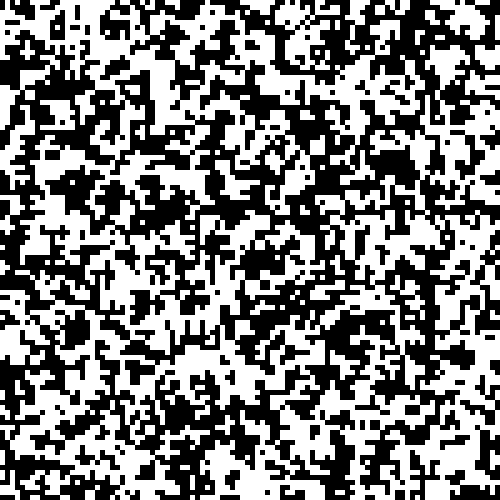
\includegraphics[width=\textwidth]{c:/users/alexander/graphics/dissVDF2T1.PNG}
    \caption{The same simulation (left) after fixation (250000 ticks) [see Section 4 for an explanation of the term 'ticks'].}
  \end{minipage}
\end{figure}

\section{Fixation in the one-dimensional vec. Deff. \\ Model}

In this section we will derive a sufficient condition for the fixation of the one-dimensional vec. Deff. Model started from a product measure, where each feature $i \in \{1,2,...,F\}$ of each individual $x \in \mathbb{Z}$ is independently given the configuration 1 with probability $p \in ]0,1[$ , i.e. $P(\tilde{\eta}_{0}(x,i)=1)= p$. The following Lemma, which gives a sufficient condition for fixation, was first proven for cyclic particle systems in \cite{Griffeath89} and more recently extended to the vec. Deff. Model in \cite{ClustCoex}. We will elaborate on the proof of this Lemma and then proceed to derive a further sufficient condition for fixation, which is weaker but easier to work with. In Section 5.1 we define the contribution variable, which establishes a link between the fixation event in Lemma 5.1. and the distribution of particles from the symmetric annihilating random walks. In Section 5.2 we define the weight function, which is defined to be a stochastic approximation of the contribution variable and derive a sufficient condition for fixation based on the expected value of the weight function. Lastly, Section 5.3 is devoted to deriving fixation for various parameter values ($F$ and $\theta$) in one dimension by studying the behaviour of the weight function. The whole of Section 5 is an extension of Lanchier's work in \cite{ClustCoex}, where he considered the system started from a product measure with $p=\frac{1}{2}$.

\begin{lemma}
For all $(z,i) \in \mathbb{Z}\times \{ 1,2,...,F \}$, let
\begin{equation}
T(z,i) := \inf \{ t: (z,0) \rightsquigarrow^i (0,t)\}.
\end{equation}
Then the vec. Deff. Model fixates whenever
\begin{equation}
\lim_{N \rightarrow \infty} P(T(z,i)< \infty \text{ for some } z<-N \text{ and } i=1,2,...,F) = 0.
\end{equation}
\end{lemma}

By reflection symmetry of the system, this means that if the probability that the person at the origin is influenced by persons increasingly far away from the origin in finite time diminishes to zero, the system fixates a.s..

\begin{proof}
The proof relies on the translation invariance of the system. It is proven that almost surely the individual at the origin does not change her configuration after a fixed finite time, implying that the system itself fixates. \\ 
For each $i \in \{ 1, ..., F \}$ we define a collection of stopping times $(\tau_{i,j})_{j \in \mathbb{N}}$, where 
\begin{equation}
\tau_{i,0}:= 0, \: \tau_{i,j}:= \inf \{ t > \tau_{i,j-1} : \tilde{\eta_t}(0,i) \neq \tilde{\eta}_{\tau_{i,j-1}}(0,i) \} \text{ for } j \geq 1,
\end{equation}
i.e. $\tau_{i,j}$ is the $j^{th}$ time the individual at the origin changes her $i^{th}$ attribute. We define the random variables $a_{i,j}$, where
\begin{equation}
a_{i,j} := \{z \in \mathbb{Z}: \text{there exists an active $i$-path } (z,0) \rightsquigarrow^i (0,\tau_{i,j})\}.
\end{equation}
$a_{i,j}$ is the \textit{ancestor} of vertex 0 at time $\tau_{i,j}$ for the $i^{th}$ feature and $a_{i,j} \in \mathbb{Z}$. Due to the definition of active $i$-paths and a simple induction, the $i^{th}$ feature of vertex $0$ at time $\tau_{i,j}$ is equal to the initial value of the $i^{th}$ feature of vertex $z$. So we call vertex $z$ the (unique) \textit{ancestor} of vertex $0$ at time $\tau_{i,j}$ for the $i^{th}$ feature. \\
And we define the events $B_i$ and $G_{i,N}$, where
\begin{equation}
B_i := \{ \tau_{i,j}< \infty \text{ for all } j \} \text{ and } G_{i,N} := \{ \vert a_{i,j}\vert < N \text{ for all } j \}.
\end{equation}

The assumption that $\lim_{N \rightarrow \infty} P(T(z,i)< \infty \text{ for some } z<-N \text{ and } \\ i=1,2,...,F) = 0$ together with the reflection symmetry implies that for each cultural feature $i$, the event $G_{i,N}$ occurs almost surely for some $N$. Furthermore, the event that the individual at the origin changes his configuration infinitely often, implies that $B_i$ occurs for at least one feature $i \in \{1,2,...,F\}$. It holds that
\begin{equation}
\begin{split}
P(\bigcup_{1 \leq i \leq F}B_i) & \leq \underset{1 \leq i \leq F}{\sum}P(B_i) \leq \underset{1 \leq i \leq F}{\sum} P(B_i \cap (\underset{N}{\bigcup}G_{i,N})) \\ = & \underset{1 \leq i \leq F}{\sum}P(\underset{N}{\bigcup} (B_i \cap G_{i,N})).
\end{split}
\end{equation}

Hence, in order to establish fixation, it suffices to prove that $P(B_i \cap G_{i,N})=0$ for all $i \in \{1,2,...,F\}$ and all $N\geq 1$. We prove that this holds with an application of the martingale convergence theorem.\
Define the continuous time process $I_t(x,i)$, where $t\geq 0$, $x\in \mathbb{Z}$ and 
\begin{equation}
\begin{split}
I_t(x,i)&:= \{ z \in \mathbb{Z}: (z,i) \text{ is the ancestor of } (x,i) \text{ at time } t \}. \\
& \text{Let} \\
M_t(x,i) & := \vert I_t(x,i) \vert.
\end{split}
\end{equation}
Since each interaction between two individuals is equally likely to effect the culture of each of the the two individuals, $M_t(x,i)$ the number of descendants of any given site is a martingale whose expected value is constantly equal to one ($E(M_t(x,i))\equiv 1$) [analogous to proof of Lemma 3.2.]. Hence, it follows from the martingale convergence theorem that $\lim_{t \rightarrow \infty} M_t(x,i) = M_{\infty}(x,i)$ almost surely, where $E\vert M_{\infty}(x,i) \vert < \infty$. Thus, for almost all realizations of the process, the number of descendants of $(x,i)$ converges to a finite value in finite time. It holds that 
\begin{equation}
s(x,i) := \inf \{ t>0 : M_t(x,i) = M_{\infty}(x,i) \}< \infty \text{ almost surely}.
\end{equation}
Simultaneous updates, depending on jump times of independent Poisson processes, occur with probability zero. Thus, a space-time point $(x,i)$ cannot win and lose and ancestor at the same time. It follows that the set of descendants, $I_t(x,i)$, inherits the convergence properties of $M_t(x,i)$:
\begin{equation}
\lim_{t \rightarrow \infty} I_t(x,i) = I_{\infty}(x,i) \text{  and  } r(x,i) := \inf \{ t>0 : I_t(x,i) = I_{\infty}(x,i) \}< \infty \text{ a.s.},
\end{equation}
where, due to one dimensional nearest neighbour interactions, $I_{\infty}(x,i)$ is a random interval which is almost surely finite. \\
Conditional on the event $G_{i,N}$, for arbitrary $N \in \mathbb{N}$, the last time the individual at the the origin changes the configuration of her $i^{th}$ feature is no greater than $\max \{ r(x,i): x \in (-N,N) \}$. And it follows that
$$ P(B_i \cap G_{i,N}) = P(r(x,i) = \infty \text{ for some } x \in (-N,N))=0. $$ 
\end{proof} 

We now proceed to quantify the event $\{ T(z,i) < \infty: \text{ for some }z< -N \text{ and} \\ \text{ some } i=1,2,...,F  \}$ for given $N \in \mathbb{N}$. 

\subsection{The `contribution' variable}

To derive a further sufficient condition for fixation which is easier to work with, we use the notion of generalized active paths to "[...] construct a random interval such that all the blockades initially in the interval must have been destroyed by either active particles initially in this interval or active particles that result from the destruction of these blockades." \cite[p. 552]{ClustCoex} Here, for given $N \in \mathbb{N}$, we define the key event $H_N$ s.t.
\begin{equation}
H_N := \{ T(z,i) < \infty: \text{ for some }z< -N \text{ and some } i=1,2,...,F  \}.
\end{equation}
Let $T_N:= \inf \{ T(z,i): z < -N \text{ and } i=1,2,...,F\}$ be the first time that an active $i$-path originating from left of $-N$ hits the origin. Then it holds that 
\begin{equation}
H_N = \{ T_N < \infty \}.
\end{equation}
Conditional on the event $H_N$ we construct space-time interval which will undergo a net loss of particles. Let $z^*$ be s.t. $T(z^*,i)=T_N$ and let 
\begin{equation}
\begin{split}
z_- & := \min \{ z \in \mathbb{Z}: (z,0) \rightsquigarrow (0,T_N) \} \leq z^* < -N \text{ and}\\
z_+ & := \max \{ z \in \mathbb{Z}: (z,0) \rightsquigarrow (0,S) \text{ for some } S<T_N \} \geq 0,
\end{split}
\end{equation}
where $\rightsquigarrow$ now denotes a generalized active path. And let $I_N:= (z_-, z_+)$.\
Since generalized active paths cannot cross a blockade, it follows that $I_N$ has the following two properties:
\begin{enumerate}
\item All blockades initially in $I_N$, must have been destroyed by the time $T_N$.
\item None of the active paths can cross the outer generalized active paths defined by $I_N$ from either direction. Hence, active particles initially outside $I_N$ cannot jump into the space-time interval delimited by the two generalized active paths $(z_-,0) \rightsquigarrow (0,T_N)$ and ($z_+,0) \rightsquigarrow (0,S)$ defined above. 
\end{enumerate}
Hence, $I_N$ gives a suitable interval. \\
Next, we define a collection of random variables to quantify the event $H_N$. We call these random variables the \textbf{contribution} of particles to an edgde, as in \cite{ClustCoex}, where $cont: E(\mathbb{Z}) \rightarrow \mathbb{Z}$ ($E(\mathbb{Z})$ denotes the edge set of the $\mathbb{Z}$-lattice). The contribution variable "[...] counts particles using different weights: particles initially active that become frozen are counted positively while particles initially frozen that become active are counted negatively. In addition, particles initially active that annihilate are counted positively if the annihilation is the result of their jump but negatively otherwise, so that overall pairs of active particles that annihilate do not contribute."\cite[p.553]{ClustCoex} Formally we define: \\
If $e$ is initially a \textbf{blockade},
\begin{equation}
\begin{split}
cont(e)&:= \#\{\text{active particles that either annihilate or become frozen as a result} \\
 & \text{of a jump onto $e$ before $e$ becomes an active edge } \} -  \\
 & \#\{ \text{particles initially at $e$ that ever become active} \}.
\end{split}
\end{equation}
If $e$ is initially an \textbf{active} edge,
\begin{equation}
\begin{split}
cont(e)&:= \#\{\text{active particles that either annihilate or become frozen as a result} \\
 & \text{of a jump onto $e$ before the first jump of an active particles initially at $e$} \}   \\
 & - \#\{\text{particles initially at $e$} \}.
\end{split}
\end{equation}
On the event $H_N$, all blockades initially in $I_N$ must be destroyed in finite time by active particles initially in $I_N$ or active particles that resulted from a destruction of such a blockade. Hence, there are no particles initially frozen that remain frozen and are also not accounted for in definition of the contribution. The event $H_N$ implies that a particle on level $i$ jumps from left of the edge $(-N-1)(-N)$ towards and across the origin. By recalling properties (1) and (2) of $I_N$ we deduce, for all $i \in \{ 1,2,...,F \}$, 
\begin{equation}
\begin{split}
& H_N = \{T_N < \infty \} \subseteq \{ \underset{e \in I_N}{\sum}cont(e) \leq 0 \} \\
& \Rightarrow \{ \underset{e \in I_N}{\sum}cont(e) > 0  \} \subseteq \{ T_N= \infty \}.
\end{split}
\end{equation}

It follows that a positive sum of contributions over the interval $I_N$, for some $N \in \mathbb{N}$, implies fixation. Before we formulate a further sufficient condition for fixation, we define an approximation of the contribution variable.

\subsection{The `weight' function}

The weight function, as it is named in \cite{ClustCoex} is an explicit random function $\phi: E(\mathbb{Z}) \rightarrow \mathbb{Z}^{\Omega}$  defined to be stochastically smaller that the contribution variable. The aim is to find a random function such that $\{E(\phi(e))> 0\} \subseteq \{ T_N= \infty \} $, for any $e \in E(\mathbb{Z})$, and thus obtain a less demanding sufficient condition for fixation. This will follow from standard large deviation estimates. \\
\indent The central assumption we make is that 
\begin{itemize}
\item[\textbf{(*)}] the initial distribution and dynamics of the model are invariant by permutation of the levels, i.e. the vertical order of the features in the representation using annihilating particles.
\end{itemize}
This assumption does not really pose any restraints, and includes the product measure of our initial configuration, since this includes all initial distributions where $P(\eta_0(x)=u)=P(\eta_0(x)=v) \text{ for all } u,v \in \Gamma \text{ with } H(u,0)=H(v,0)$. \\
It follows with the assumption \textbf{(*)} that the first jump of an active particle onto a blockade (an edge $e$ s.t. $\zeta_0(e)=j \geq \theta$) is equally likely to occur at each level and results in
\begin{itemize}
\item an annihilating event with probability $j/F$ or
\item a blockade increase -- extra particle on the edge -- with probability $1-j/F$.
\end{itemize}
We define the weight function $\phi$ s.t.
\begin{equation}
\begin{split}
&\phi: E( \mathbb{Z} )\rightarrow \mathbb{Z}^{\Omega}, \\
&\phi(e):= \left\{\begin{array}{cl} -j, & \mbox{ if } \zeta_0(e)=j \leq \theta, \\ 
j + 2(X_{e,j}-\theta), & \mbox{ if } \zeta_0(e)=j > \theta \end{array}\right.
\end{split}
\end{equation}
where $X_{e,j} := Bernoulli(1-j/F)$ and $(X_{e,j})_{e \in E(\mathbb{Z}), 1\leq j \leq F}$ independent.

\begin{lemma}
The weight $\phi(e)$ is stochastically smaller than the contribution $cont(e)$ ($\phi(e)\preceq cont(e)$) for all edges $e \in I_N$ and $N \in \mathbb{N}$.
\end{lemma}
This a corrected version of the Lemma 4.2. in \cite{ClustCoex}, where $\phi(e)\preceq cont(e)$ is stated to hold for any edge $e \in E(\mathbb{Z})$.

\begin{proof}
Let $e \in I_N$ and $\zeta_0(e)=j$ be the number of particles initially at $e$. \\
\underline{If $j \leq \theta$}, then $e$ is initially an active edge and it follows from the definition of variable $cont$ that almost surely
$$cont(e) \geq - \#\{ \text{particles initially at e} \}= -j.$$
\underline{If $j > \theta$}, then $e$ is a blockade initially and $j-\theta$ particles are needed to break the blockade which in turn results in $\theta$ particles initially frozen becoming active. Since there are no particles in $I_N$ which are initially frozen and remain frozen, it holds that 
$$ cont(e) \geq (j- \theta)-\theta = j -2\theta.$$
The event of a blockade increase, i.e. an active particle becoming frozen as the result of a jump onto $e$ before $e$ becomes an active edge, occurs with probability $1-j/F$. In the event of a blockade increase 2 additional particles must annihilate before the edge becomes an active edge. So the weight $\phi(e)$ approximates $cont(e)$ from below by taking into account the event of the first jump onto the edge and it holds that
$$cont(e) \geq (1-X_{e,j})(j-2\theta)+ X_{e,j}(j-2\theta +2)= j + 2(X_{e,j}-\theta),$$
where $X_{e,j} := Bernoulli(1-j/F)$.
\end{proof}

The central result to be derived in Theorem 5.7. is that a positive expected value of the weight function implies fixation. But before we can make large deviation estimates for $E\phi(e)$ we must make large deviation estimates for the number of $j$-edges -- the number of edges with $j$ particles.
To ease notation, in the following two sections we will derive large deviation estimates for the interval $[-N,0]$ and not $I_N$. Note that $[-N,0] \subseteq I_N$, by definition, and that the estimates also hold for any interval $[r,l]_{r \leq-N,l \geq 0}$ if $N$ is replaced by the length $\vert r-l \vert $ in the estimating functions.

\subsubsection{Large deviation estimates for number of j-edges}

Starting from a product measure such that $P(\tilde{\eta}_{0}(x,i)=1)= p \in ]0,1[$ for all $i$ and $x$ independently, the configuration at two adjacent sites on a given level are either different with probability $2p(1-p)=:\hat{p}$ or equal with probability $(p^2+(1-p)^2)=1-\hat{p}$. Which implies that the initial number of particles at any given edge is a binomial random variable:
\begin{equation}
P(\eta_0(e)=j)= \binom{F}{j} \hat{p}^j (1-\hat{p})^{F-j} \text{ for each edge e. }
\end{equation}
However, the problem we are confronted with, which does not appear for the case $p=\frac{1}{2}$ (this is the case dicussed in \cite{ClustCoex}), is that the number of particles at adjacent edges are not independent. For example, in the 1-Feature case we have that \\
$P(\text{two adjacent egdes both have a particle})= p^2(1-p)+p(1-p)^2,$ whereas, \\
$[P(\text{there is a particle on edge e})]^2= 4p^2(1-p)^2$.
A different approach is needed. We must approximate the distribution of particles. \\
\indent Let $p_u := P(\eta_0(x)=u)= p^{H(u,0)}(1-p)^{F-H(u,0)}$ denote the density of initial configuration for $u \in \Gamma$, and let
\begin{equation}
e_N(u,v):= \vert \{ x \in [-N,0]: \eta_0(x)=u \text{ and } \eta_0(x+1)=v \} \vert,
\end{equation}
denote the number of edges connecting individuals with configuration $u$ and $v$.  \\
Consider a collection of independent random variables $(Y_k)_{k \in -\mathbb{N}} \sim Bernoulli(p_u)$, such that for each $x \in [-N,0] \text{ it holds that } P(\eta_0(x)=u)= P(Y_{x}=1)= p_u $. And denote the number of \textit{changeovers}, i.e. the number of adjacent vertices pairs where exactly one vertex has the configuration $u$, by
$$ Z_N := \underset{k \in [-N.0]}{\sum}1_{\{Y_{k-1} \neq Y_k \}} .$$
Then the expected value is
$$ EZ_N = \underset{k \in [-N.0]}{\sum} E 1_{\{Y_{k-1} \neq Y_k \}} = \underset{k \in [-N.0]}{\sum}P( Y_{k-1} \neq Y_k ) = Np_u(1-p_u).$$
The following large deviation estimate holds for the number of \textit{changeovers}. We do not revise the proof here.

\begin{lemma}[\cite{FluxvsFix} Lemma 7.]
For all $\epsilon>0$, there exists a constant $c_0>0$ and $N_0 \in \mathbb{N}$ such that 
$$ P(Z_N - EZ_N \not\in (-\epsilon N, \epsilon N )) \leq \exp(-c_0 N),$$ for all $N > N_0$.
\end{lemma}

Given this large deviation estimate, we can deduce a large deviation estimate for the number of edges of each type $e_N(u,v)$.

\begin{lemma}
For all $\epsilon>0$, there exists $c_1>0$ and $N_1 \in \mathbb{N}$ such that
$$P(e_N(u,v) -Np_up_v \not\in (- \epsilon N, \epsilon N)) \leq 4\exp(c_1N)$$
for all $N > N_1$ and $u\neq v \in \Gamma$.
\end{lemma}
\begin{proof}
The proof follows the proof of Lemma 8. in \cite{FluxvsFix}. If we fix the configuration $u$, it holds that the sum of all edges bordered by a site with the configuration $u$ and a site with configuration $\neq u$ is equal to the number of \textit{changeovers}: $\underset{v:v \neq u}{\sum}e_N(u,v)= Z_N$. Hence, with the previous Lemma it follows that
\begin{equation}
P(\underset{v:v \neq u}{\sum}e_N(u,v) - Np_u(1-p_u)  \not\in (-\epsilon N, \epsilon N )) \leq \exp(-c_0 N),
\end{equation} 
for $N$ sufficiently large. Furthermore, each site with configuration $u$ preceding a changeover is followed independently by a site with any of $2^F-1$ configurations. Hence, 
\begin{equation}
\begin{split}
\text{conditional on }\underset{v:v \neq u}{\sum}e_N(u,v)=K \text{, it holds that } \\
e_N(u,v) \sim Binomial(K,p_v(1-p_u)^{-1}),
\end{split}
\end{equation}
where $(1-p_u)^{-1}$ is a normalizing factor of the conditional density. 
Letting $K^+_{\epsilon} := Np_u(1-p_u) + \epsilon N$ and $K^-_{\epsilon} := Np_u(1-p_u) - \epsilon N$, we estimate in two steps. Using the previous Lemma and large deviation estimates for the binomial distribution\footnote{If $Z \sim Binomial(N,p)$ it holds that: $P(Z \leq Np - \epsilon N ) \leq \exp(-\frac{1}{2} N p^{-1} \epsilon^2)$ and $P(Z \geq Np + \epsilon N ) \leq \exp(-\frac{1}{2} N (1-p)^{-1} \epsilon^2)$ for all $\epsilon>0$.}, for all $\epsilon^*>0$ there exists a constant $b$ s.t. $0<b<\frac{\epsilon^*(2-p_v(1-p_u)^{-1})}{p_u(1-p_u)+\epsilon^*}$ and a constant $ c_2 > 0$ such that
\begin{equation}
\begin{split}
&P(e_N(u,v) -Np_up_v \geq 2 \epsilon^* N) \leq P(\underset{v:v \neq u}{\sum}e_N(u,v)-Np_u(1-p_u) \geq \epsilon^* N) \\
& + P(e_N(u,v) \geq Np_up_v +2 \epsilon^* N \vert \underset{v:v \neq u}{\sum}e_N(u,v)-Np_u(1-p_u) < \epsilon^* N) \\
& \leq \exp(-c_0N) + P(Binomial(K^+_{\epsilon^*},p_v(1-p_u)^{-1}) \geq Np_up_v + 2 \epsilon^* N) \\
&\leq \exp(-c_0N) \\
& + P(Binomial(K^+_{\epsilon^*},p_v(1-p_u)^{-1}) \geq K^+_{\epsilon^*} (p_v(1-p_u)^{-1} + b)) \\
& \leq \exp(-c_0N) + \exp(-\frac{b^2}{2 (1-p_v(1-p_u)^{-1})} K^+_{\epsilon^*}) \\
& \leq \exp(-c_0N) + \exp(-c_2N),
\end{split}
\end{equation}
for sufficiently large $N$.\\
Analogously, for all $\epsilon^*>0$ there exists a constant $c_3>0$ such that
\begin{equation}
P(e_N(u,v)) -Np_up_v \leq -2 \epsilon N)\leq \exp(-c_0N) + \exp(-c_3N),
\end{equation}
for sufficiently large $N$. \\
The Lemma then follows by setting $\epsilon^*= \epsilon/2$ and $c_1 \leq \min\{c_0,c_2,c_3\}$.
\end{proof}

We can now formulate a large deviation estimate for the number of $j$-edges.

\begin{lemma}
For all $\epsilon>0$ and $j \in \{1,2,...,F\}$ there exist constants $c_4>0$, $C>0$ such that
$$P(e_N(j)-Np_j \not\in (-\epsilon N, \epsilon N)) \leq C\exp(-c_4N),$$
for large $N$.
\end{lemma}

\begin{proof}
To finally deduce a large deviation estimate for the initial number of edges with $j$-particles, we note that for an \textit{edge with $j$-particles on fixed levels} there are exactly $2^F$ `edge-configurations', $(u,v) \in \Gamma^2$, such that $H(u,v)= j \in \{1,2,...,F\}$. Let $U_j:=\{(u,v)\in \Gamma^2: H(u,v)=j)\}$ be the set of all `edge-configurations' such that the connecting edge has $j$-particles on arbitrary levels. This set is of cardinality $\vert U_j \vert = 2^F\binom{F}{j}$.
For $e_N(j):= \#\{ \text{edges in $[-N,0]$ with $j$ particles}\}$ it holds that 
\begin{equation}
\begin{split}
&e_N(j) = \sum_{(u,v) \in U_j}e_N(u,v) \\
& \text{and } p_j = 2^F\binom{F}{j}(p_u p_v), \text{ for any } (u,v)\in U_j,
\end{split}
\end{equation}
where again the invariance by permutation of levels is assumed. \\
Let $\epsilon >0 $, $j \in \{1,2,...,F\}$ and sufficiently large $N$, it then follows that
\begin{equation}
\begin{split}
&P(e_N(j)-Np_j \not\in (-\epsilon N, \epsilon N)) \\
&=P(\sum_{(u,v) \in U_j}e_N(u,v) -N2^F\binom{F}{j}p_u p_v \not\in (-\epsilon N, \epsilon N)) \\
&=P(\sum_{(u,v) \in U_j}[e_N(u,v) -Np_u p_v] \not\in (-\epsilon N, \epsilon N)) \\
& \leq \sum_{(u,v) \in U_j}P(e_N(u,v) -Np_u p_v \not\in (-\epsilon N, \epsilon N)) \\
& \leq 4\cdot 2^F\binom{F}{j}\exp(-c_4N)=:C\exp(-c_4N).
\end{split}
\end{equation}
For each summand there exists an approximating constant $c^{(u,v)}_1$  according to Lemma 5.4.. $c_4:= \min\{c^{(u,v)}_1: (u,v) \in U_j \}$. 
\end{proof}
In next section we derive a large deviation estimate for the total weight over $(-N,0)$, i.e. $\sum_{e\in (-N,0)}\phi(e)$, before finally proving our fixation Theorem.

\subsubsection{Large deviation estimates for the weight}

\begin{lemma}
For all $\epsilon>0$, there exist constants $c_7>0$,$C_0>0$ (depending on $F$) such that
$$P((\sum_{e\in (-N,0)}\phi(e)-NE\phi(e)) \not\in (-\epsilon N, \epsilon N)) \leq C_0\exp(-c_7N),$$
for large $N$ and any $e  \in E(\mathbb{Z})$.
\end{lemma}
\begin{proof}
The expectation of the random function $\phi(e)$ is given by: 
\begin{equation}
\begin{split}
E\phi(e) &= \sum_{j \leq \theta}(-j)p_j + \sum_{j>\theta}(j+2(1-\frac{j}{F}-\theta))p_j \\
&= \sum_{j \leq \theta}(-j)p_j + \sum_{j>\theta}(j-2\theta)p_j + \sum_{j>\theta}2(1-\frac{j}{F})p_j.
\end{split}
\end{equation}
Using the notation of the previous two section and letting
$$\Omega_j := \{ e \in (-N,0): \zeta_0(e)=j \} \text{ for } 1\leq j \leq F,$$
we can express the random weight of the interval $(-N,0)$ as
\begin{equation}
\begin{split}
\sum_{e\in (-N,0)}\phi(e)& = \sum_{j \leq \theta}(-j)e_N(j) + \sum_{j > \theta}(j+ 2(X_{e,j}-\theta))e_N(j) \\
&= \sum_{j \leq \theta}(-j)e_N(j) + \sum_{j > \theta}(j- 2\theta)e_N(j)+ \sum_{j>\theta}\sum_{e \in \Omega_j}2X_{e,j}. \\
\end{split}
\end{equation}
Hence, we deduce that
\begin{equation}
\begin{split}
&P((\sum_{e\in (-N,0)}\phi(e)-NE\phi(e)) \not\in (-\epsilon N, \epsilon N)) \leq \\
&\; \sum_{j \leq \theta}P((-j)(e_N(j)-Np_j) \not\in (-\epsilon N, \epsilon N)) \\
&+\sum_{j>\theta}P((j-2\theta))(e_N(j)-Np_j) \not\in (-\epsilon N, \epsilon N)) \\
&+\sum_{j>\theta}P((\sum_{e \in \Omega_j}2X_{e,j}-2(1-\frac{j}{F})Np_j) \not\in (-\epsilon N, \epsilon N))\\
&=:\textbf{(i)+(ii)+(iii)}.
\end{split}
\end{equation}

The summands of terms \textbf{(i)-(ii)} can now be easily estimated using the final result of the previous section. It holds that
\begin{equation}
\textbf{(i)} \leq \sum_{j \leq \theta}P((e_N(j)-Np_j) \not\in (-\frac{\epsilon}{F} N, \frac{\epsilon}{F} N))\leq \theta C\exp(-c_4 N)
\end{equation}
and
\begin{equation}
\textbf{(ii)} \leq \sum_{j>\theta} P((e_N(j)-Np_j) \not\in (-\frac{\epsilon}{2F} N, \frac{\epsilon}{2F} N))\leq (F-\theta)C\exp(-c_4 N),
\end{equation}
where $c_4$ and $C$ represents the minimum and maximum respectively of all estimating constants. Lemma 5.5. gives the existence of estimating constants for each summand. \\
To estimate the summands \textbf{(iii)} we use standard large deviation estimates for binomial random variables, since $(X_{e,j})_{e \in E(\mathbb{Z})}$ are independent Bernoulli random variables. Let $Z$ be a binomial random variable such that $Z \sim Binomial(N(p_j + \epsilon/4),1-\frac{j}{F})$. There exists a $c_5>0$ depending on $j$ such that
\begin{equation}
\begin{split}
&P(\sum_{e \in \Omega_j} 2X_{e,j}-2(1-\frac{j}{F})Np_j \leq -\epsilon N)  \\
&=P(\sum_{e \in \Omega_j} X_{e,j}-(1-\frac{j}{F})Np_j \leq -\frac{\epsilon}{2} N)\\
&\leq P(\sum_{e \in \Omega_j} X_{e,j}-(1-\frac{j}{F})Np_j \leq -\frac{\epsilon}{2} N \vert e_N(j) < N(p_j + \frac{\epsilon}{4})) + \\
&\;\;\; P(e_N(j) \geq N(p_j + \frac{\epsilon}{4}))\\
&\leq P(\sum_{e \in \Omega_j} X_{e,j}-(1-\frac{j}{F})Np_j \leq -\frac{\epsilon}{2} N \vert \vert\Omega_j\vert = N(p_j + \epsilon/4)) + C\exp(-c_4N) \\
&\leq P(Z -(1-\frac{j}{F})Np_j \leq -\frac{\epsilon}{2} N ) + C\exp(-c_4N)\\
&\leq P(Z -(1-\frac{j}{F})N(p_j+ \epsilon/4) \leq -\frac{\epsilon}{2}N-(1-\frac{j}{F})\frac{\epsilon}{4}N)+ C\exp(-c_4N) \\
&= P(Z -(1-\frac{j}{F})N(p_j+ \epsilon/4) \leq -\frac{\epsilon}{4}(3-\frac{j}{F})N) + C\exp(-c_4N) \\
& \leq \exp(-\frac{1}{2}(\frac{\epsilon}{4}(3-\frac{j}{F}))^2(1-\frac{j}{F})^{-1}N)+C\exp(-c_1N)\\
&:= \exp(-c_5N)+C\exp(-c_4N).
\end{split}
\end{equation}
Similarly, for all $\epsilon>0$ there exists a constant $c_6>0$ depending on $j$ s.t.
\begin{equation}
P((\sum_{e \in \Omega_j} 2X_{e,j}-2(1-\frac{1}{F})Np_j \geq \epsilon N) \leq \exp(-c_6N)+C\exp(-c_4N).
\end{equation}
Since we have estimates for each summand of a finite sum, it follows that there exist constants $C_0$ and $c_7>0$ s.t.
\begin{equation}
\begin{split}
&P((\sum_{e\in (-N,0)}\phi(e)-NE\phi(e)) \not\in (-\epsilon N, \epsilon N)) \leq C_0\exp(-c_7N).
\end{split}
\end{equation}
where $c_7$ denotes the minimum over all estimating constants in the exponent and $C_0$ the sum of all coefficients.
\end{proof}

We have now completed all large deviation estimates and can derive the central result of this section.

\begin{theorem}
The system fixates whenever $E\phi(e)>0$.
\end{theorem}

\begin{proof}
Simply to recall the events under consideration, we have
$$H_N = \{ T(z,i) < \infty: \text{ for some }z< -N \text{ and some } i=1,2,...,F  \}$$
and it holds that
\begin{equation}
\begin{split}
& H_N  \subseteq \{ \underset{e \in I_N}{\sum}cont(e) \leq 0 \}\overset{\phi(e) \preceq cont(e)}{\subseteq} \{ \underset{e \in I_N}{\sum}\phi(e) \leq 0 \} \\
&\overset{Def. \: I_N}{\subseteq} \{ \underset{e \in [l,r]}{\sum}\phi(e) \leq 0 \text{ for some } l<-N \text{ and some }r \geq 0 \}.
\end{split}
\end{equation}

Let $\epsilon := E\phi(e)>0$. Then, according to Lemma 5.6., there exist constants $c_7>0$, $C_0$ s.t.
\begin{equation}
P(\sum_{e \in (-N,0)}\phi(e) \leq 0 ) = P(\sum_{e \in (-N,0)}\phi(e) \leq N(E\phi(e)- \epsilon)) \leq C_0\exp(-c_7N).
\end{equation}

Hence, it follows from the large deviation estimates that
\begin{equation}
\begin{split}
& \lim_{N \rightarrow \infty}P(H_N) \leq \lim_{N \rightarrow \infty}P(\underset{e \in I_N}{\sum}cont(e) \leq 0) \\
&  \leq \lim_{N \rightarrow \infty}P(\underset{e \in I_N}{\sum}\phi(e) \leq 0) \\
&  \leq \lim_{N \rightarrow \infty}P(\underset{e \in [l,r]}{\sum}\phi(e) \leq 0 \text{ for some } l<-N \text{ and some }r \geq 0) \\
&  \leq \lim_{N \rightarrow \infty}\sum_{l < -N}\sum_{r \geq 0}P(\underset{e \in [l,r]}{\sum}\phi(e) \leq 0) \\
&  \leq \lim_{N \rightarrow \infty}\sum_{l < -N}\sum_{r \geq 0}C_0\exp(-c_6  \vert r-l \vert) =0.
\end{split}
\end{equation}
Fixation then follows from Lemma 5.1..
\end{proof}

As noted above, Theorem 5.7. is a version (a somewhat weaker version) of Lemma 5.1. from which it is easier to derive fixation for specific parameters. And this is the purpose of the following section.

\subsection{Parameters leading to fixation}

We first list some basic properties of $E\phi(e): [0,1] \rightarrow \mathbb{R}$ as a function with argument $p \in [0,1]$ where 
$$E\phi(e)(p) = \sum_{j \leq \theta}(-j)p_j(p) + \sum_{j>\theta}(j+2(1-\frac{j}{F} - \theta ))p_j(p)$$ 
and 
$$p_j(p) = \binom{F}{j}(2p(1-p))^j(p^2+(1-p)^2)^{F-j}.$$ 

It holds that: 
\begin{itemize}
\item $E\phi(e)$, as a finite power series, is continuous differentiable in $p$.
\item $E\phi(e)(p)=0$ for $p\in\{0,1\}$, so Theorem 5.7. can be extended to trivial product measures, since the systems clusters almost surely at time $t=0$ when started from trivial product measures.
\item\ $\frac{dE\phi(e)}{dp} = \sum_{j \leq \theta}(-j)\frac{d}{dp} p_j + \sum_{j>\theta}(j+2(1-\frac{j}{F}-\theta))\frac{d}{dp} p_j$ where 
\begin{equation}
\begin{split}
\frac{d}{dp} p_j &= \frac{d}{dp}\binom{F}{j}(2p(1-p))^j(p^2 + (1-p)^2)^{F-j} \\
&= \binom{F}{j}j(2p(1-p))^{j-1}(2-4p)(p^2 + (1-p)^2)^{F - j}\\
& + \binom{F}{j}(2p(1-p))^j(F - j)(4p - 2)(p^2 + (1-p)^2)^{F - j-1} 
\end{split}
\end{equation}
$\Longrightarrow$ 
\begin{equation}
\begin{split}
\frac{d}{dp} p_j &= 0 \\
&\Leftrightarrow j(p^2 + (1-p)^2)= (2p(1-p))(F - j)\\
&\Leftrightarrow (2(F-j)+2j)p^2-(2(F-j)-2j)p+j=0 \\
&\Leftrightarrow 2Fp^2-2Fp+j=0 \\
&\Leftrightarrow p_{1,2} = 1/2 \pm 1/2 \sqrt{(1-2j/F)} \text{ for }F \geq 2j.
\end{split}
\end{equation}
Additionally, $\frac{d}{dp} p_j = 0$ always holds for $p=1/2$ and for $p\in \{0,1\}$ if $j\neq 0,1$.
\item $\frac{dE\phi(e)}{dp}(0)=-2F$ and $\frac{dE\phi(e)}{dp}(1)=2F$.
\item $E\phi(e)$ is symmetric, i.e. $E\phi(e)(p)=E\phi(e)(1-p)$ for all $p \in [0,1]$. This follows from the symmetry of $p_j = \binom{F}{j}(2p(1-p))^j(p^2+(1-p)^2)^{F-j}$.
\item $E\phi(e) \leq 0$ for $F \leq 2\theta-1$. This follows from a simple approximation of the coefficients: 
\begin{equation}
j+ 2(1-\frac{j}{F}-\theta) \overset{j> \theta} {\leq} F+ 2(1-\frac{\theta +1}{F}-\theta)\overset{F= 2\theta -1}{\leq} -2 \frac{\theta+1}{2\theta -1} \leq 0
\end{equation}
\end{itemize}

Figure 10. and 11. depict $E\phi(e)$ for different parameter values.

\begin{figure}[h]
\centering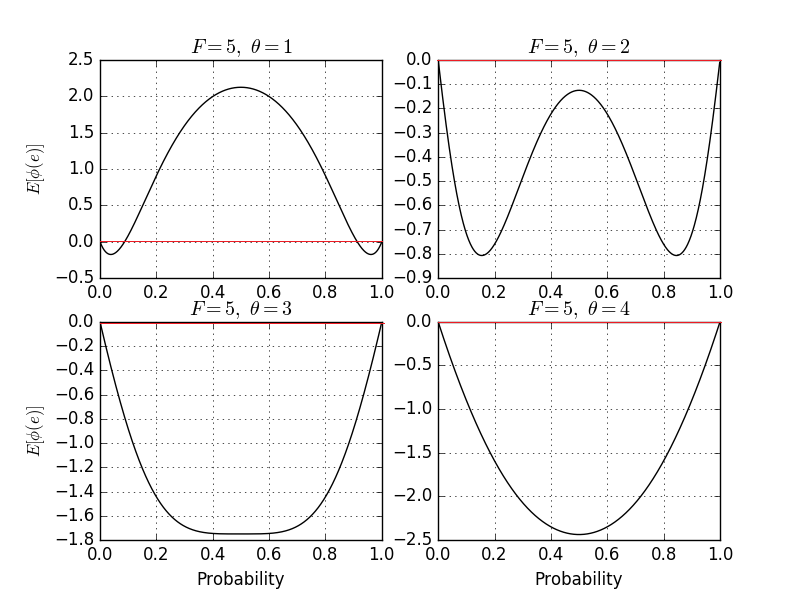
\includegraphics[width=0.6\linewidth]{c:/users/alexander/graphics/F5weight.PNG}
\caption{Graph of $E\phi(e) \vert_{[0,1]}$ for $F=5$ and a selection of thresholds. }
\end{figure}

\begin{figure}[h]
\centering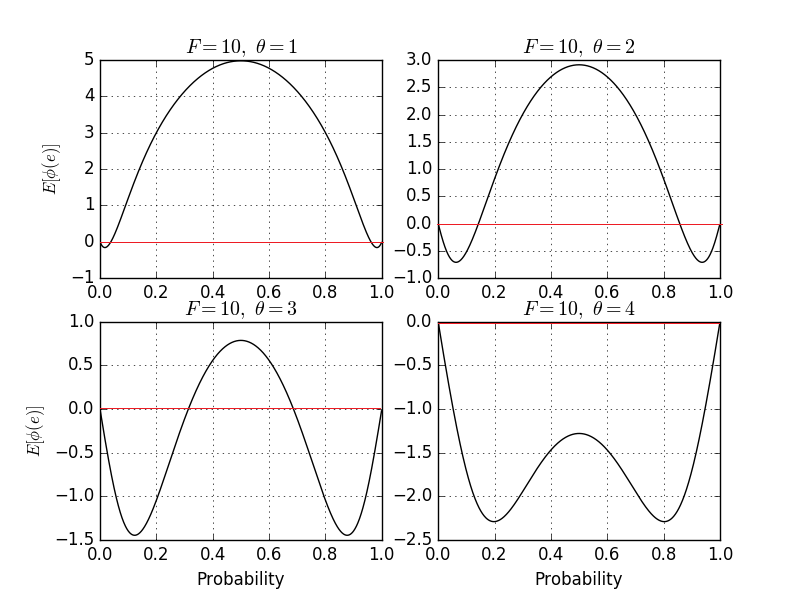
\includegraphics[width=0.6\linewidth]{c:/users/alexander/graphics/F10weight.PNG}
\caption{Graph of $E\phi(e) \vert_{[0,1]}$ for $F=10$ and a selection of thresholds. }
\end{figure}

We now seek to determine for which values of $F$, $\theta$ and $p$ it holds that $E\phi(e) > 0$ and, hence, the system fixates. We would of course expect fixation to be most probable when $F$ is much larger than $\theta$ (a low threshold). In this section we prove fixation for the cases that $F \geq 4\theta$, $F = 4\theta -1$ and $F = 4\theta-n $ where $n \in \mathbb{N}$ is odd and $n \leq 2(\theta-1)$. However, it will become clear that the case $F=3\theta$ cannot be proven with our method.

Consider the system started from a product measure with 
\begin{equation}
(\#) \text{  } P(\eta_0(x,i)=1)=p, \:\text{ for all } 1 \leq i \leq F \text{ and } \forall x\in \mathbb{Z}.
\end{equation}

\begin{lemma}
There exists an open interval $(a,1-a) \subset [0,1]$ such that the system with $F \geq 4\theta $ started from $(\#)$, fixates for all $p \in (a,1-a)$.
\end{lemma}

\begin{proof}
We prove that $E\phi(e)(\frac{1}{2})> 0$ for $F \geq 4\theta$. The existence of an open open interval $(a, 1-a)$ follows from continuity and the fact that $E\phi(e)(0)=E\phi(e)(1)=0$. The proof follows the proof of Lemma 4.5. in \cite{ClustCoex}.\\
Define the constants $K^- := \lceil \frac{1}{2}(F-1) \rceil$ and $K^+ := \lfloor \frac{1}{2}(F+1) \rfloor$. Note that $K^+ + K^- =F$ and 
\begin{equation}
F - K^- = \left\{\begin{array}{cl} K^-+1, & \mbox{ if } F \in 2\mathbb{N}+1 \\ 
K^-, & \mbox{ if } F \in 2\mathbb{N} \end{array}\right\}.
\end{equation}
Let $g_j(\theta, F) := j+2(1- \frac{j}{F}- \theta)= 2(1-\theta)+ (1-\frac{2}{F})j$, it then holds that
\begin{equation}
\begin{split}
g_{F-j}(\theta, F) &= 2(1-\theta ) +(1-\frac{2}{F})(F-j)\\
&= F-2\theta -(1-\frac{2}{F})j, \\
g_{j}(\theta, F)+g_{F-j}(\theta, F) &= F - 4\theta +2 \text{ and} \\
g_{F/2}(\theta, F) &= \frac{F}{2} -2\theta +1 \overset{F \geq 4\theta}{\geq} 1.
\end{split} 
\end{equation}
We now use the property that for $p= \frac{1}{2}$, $p_j = p_{F-j}$.\footnote{Since $\binom{n}{k}=\binom{n}{n-k} \text{ for } k \leq n$.}  It holds that
\begin{equation}
\begin{split}
&E\phi(e)(\frac{1}{2}) = \sum_{j \leq \theta}(-j)p_j + \sum_{j>\theta}(j+2(1-\frac{j}{F}- \theta ))p_j \\
& \geq \sum_{j \in \{0,1,...,\theta \}}(-j)p_j + \sum_{j>\theta} g_j(F,\theta )p_j - g_{F/2}(\theta, F)p_{F/2}\mathbf{1}_{2\mathbb{N}}(F) \\
& = \sum_{j \in \{0,1,...,\theta \}}(-j+g_{F-j}(\theta, F))p_j + \sum_{j \in \{\theta+1,\theta+2, ... ,K^- \}}(g_{j}(\theta, F) + g_{F-j}(\theta, F))p_j \\
&= \sum_{j \in \{0,1,...,\theta \}}(F-2\theta -2(1-\frac{1}{F})j)p_j + \sum_{j \in \{\theta+1,\theta+2, ... ,K^- \}}(F - 4\theta +2)p_j \\
&\geq \sum_{j \in \{0,1,...,\theta \}}(F-2\theta -2j)p_j + \sum_{j \in \{\theta+1,\theta+2, ... ,K^- \}}(F - 4\theta +2)p_j \\
& >0,
\end{split}
\end{equation}
for $F\geq 4\theta $ since all summands are strictly positive. Fixation follows from Theorem 5.7..
\end{proof}

The fixation result can be extended to the case where $F=4\theta -1$ when $\theta \geq 2$. This demands further estimation because if $F=4\theta -1$ the first sum of the previous estimation contains a negative term. 

\begin{lemma}
There exists an open interval $(a,1-a) \subset [0,1]$ such that the system with $F = 4\theta-1 $ started from $(\#)$, fixates for all $p \in (a,1-a)$.
\end{lemma}

\begin{proof}
Again, we prove that $E\phi(e)(\frac{1}{2})>0$ for the case that $F = 4\theta-1 $ and $\theta \geq 2$ making some changes to proof of Lemma 4.6. in \cite{ClustCoex}. The remaining case, namely $F=3, \theta =1$ is proven numerically. \\
Let $F=4\theta-1$, then it holds that 
\begin{equation}
\begin{split}
F-2(\theta +j) &\geq 4\theta-1 - 2(\theta+ \theta) = -1 \text{ for } j \in \{0,1,...,\theta \} \text{ and}\\
F-4\theta +2 &= 4\theta -1-4\theta +2 = 1 \text{ for } j \in \{\theta+1,\theta+2, ... ,K^- \}.
\end{split}
\end{equation}
Hence, extending the previous estimation we derive that
\begin{equation}
\begin{split}
E \phi (e)(\frac{1}{2}) &\geq \sum_{j \in \{0,1,...,\theta \}}(F-2\theta -2j)p_j + \sum_{j \in \{\theta+1,\theta+2, ... ,K^- \}}(F - 4\theta +2)p_j 
\end{split}
\end{equation}
\begin{equation}\notag
\begin{split}
&\geq \sum_{j \in \{0,1,...,\theta \}}(-1)p_j + \sum_{j \in \{\theta+1,\theta+2, ... ,K^- \}}p_j \\
&= -P(Z \in \{0,1,...,\theta \}) + P(Z  \in \{\theta+1,\theta+2, ... ,K^- \}),
\end{split}
\end{equation}
where $Z \sim Binomial(F,1/2)$ is a binomial random variable. Since $Z \in \{0,1, ..., F\}$ and $F$ is odd, the sets $\{0,1,...,\theta \},\{\theta+1,\theta+2, ... ,K^- \},\{K^+, K^++1,...,F-(\theta+1)\},\{ F-\theta ,F-\theta+1,...,F\}$ form a partition of the range of $Z$. Hence, it follows by invoking the symmetry $p_j = p_{F-j}$ (for $p0 \frac{1}{2}$) that
\begin{equation}
\begin{split}
E \phi (e) (\frac{1}{2})&= \frac{1}{2} (-P(Z \in \{0,1,...,\theta \} \cup \{ F-\theta ,F-\theta+1,...,F\}) \\
&+ P(Z \in \{\theta+1,\theta+2, ... ,K^-,K^+, K^++1,...,F-(\theta+1)\}) \\
&\geq \frac{1}{2} (1-2P(Z \in \{0,1,...,\theta \} \cup \{ F-\theta ,F-\theta+1,...,F\}) \\
&= \frac{1}{2} - 2P(Z \in \{0,1,...,\theta \}).
\end{split}
\end{equation}

We now use the standard large deviation estimate for binomial random variables, i.e.
$$ P(Z \leq F( \frac{1}{2}- \epsilon)) \leq \exp(-F\epsilon^2) \: \forall \epsilon \in ]0,\frac{1}{2} [. $$

Let $\epsilon := \frac{F/2 - \theta }{F}$. Then it holds that $0 < \frac{F/2 - \theta }{F} < \frac{1}{2}$ for $\theta>1$ and 

\begin{equation}
\begin{split}
E \phi (e)(\frac{1}{2}) &\geq \frac{1}{2} - 2P(Z \in \{0,1,...,\theta \}) \\
&= \frac{1}{2} - 2P(Z \leq \theta ) \\
&= \frac{1}{2} - 2P(Z \leq F(1/2 - \frac{F/2 - \theta }{F}) ) \\
&= \frac{1}{2} - 2P(Z \leq F(1/2 - \epsilon) ) \\
&\geq \frac{1}{2} - 2 \exp (-(4\theta-1)\epsilon^2) >0.
\end{split}
\end{equation}

It holds that $\exp (-(4\theta-1)\epsilon^2)< 1/4$ for all $\theta \geq 2$  -- see equation (81 ) in the next proof.
The numerical result for the case $F=3$ and $\theta =1 $ is depicted in Figure 12.  below.
Fixation again follows from Theorem 5.7..

\begin{figure}[h]
\centering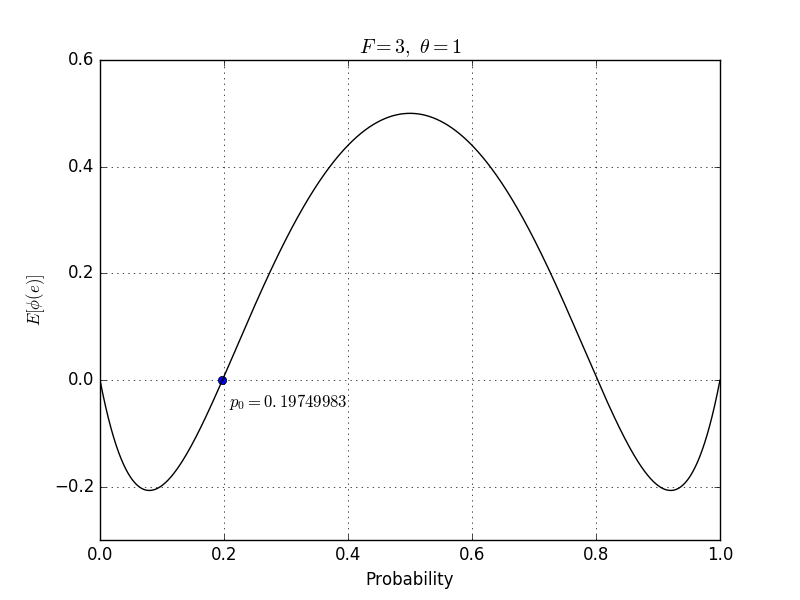
\includegraphics[width=0.7\linewidth]{c:/users/alexander/graphics/F3T1weight.PNG}
\caption{$E \phi (e)$ breaches the x-axis at $p_0$ and $1-p_0$.}
\end{figure}

\end{proof}

The proof above can be generalized to additional parameters. Note that for $\epsilon = \frac{F/2 - \theta }{F}$, the proof only demands the properties (I) $0 < \epsilon < 1/2$ and (II) $\exp(-F\epsilon^2)<1/4$.

\begin{lemma}
There exists an open interval $(a,1-a) \subset [0,1]$ such that the system with $F = 4\theta-n $ where $n \in \mathbb{N}$ is odd and $n \leq 2(\theta-1)$ started from $(\#)$, fixates for all $p \in (a,1-a)$.
\end{lemma}

\begin{proof}
The proof is analogous to the previous. Let $\epsilon := \frac{F/2 - \theta }{F}$. Then it holds that
\begin{itemize}
\item (I)
\begin{equation}
\begin{split}
& \epsilon = \frac{F/2 - \theta }{F} = \frac{(4\theta -n)/2-\theta}{4\theta -n} \leq \frac{2\theta-n}{4\theta -n} < \frac{1}{2} \\
& \text{ and is positive for } n < 2\theta,
\end{split}
\end{equation}
\item (II)
$$ \exp(-F\epsilon^2)= \exp(-F(\frac{F/2-\theta}{F})^2)=\exp(-\frac{(F/2-\theta)^2}{F}). $$
And it holds that
\begin{equation}
\begin{split}
\exp(-F\epsilon^2) &< 1/4 \\
\Leftrightarrow -\frac{((4\theta -n)/2-\theta)^2}{4\theta -n} &< \log(1/4)  \\
\Leftrightarrow \frac{(\theta -n/2)^2}{4\theta -n} &> -\log(1/4) \\
\Leftarrow (\theta -n/2)^2 &> \frac{3/2}{4\theta -n}, 
\end{split}
\end{equation}
for $\theta \geq 1$ and $n \leq 2\theta$ it holds that $\frac{3/2}{4\theta -n}<1$, and $(\theta -n/2)^2\geq 1 \Leftrightarrow 2(\theta-1)\geq n$.
\end{itemize}
Fixation again follows from Theorem 5.7..
\end{proof}

Furthermore, numerical results show that for the cases $(F=3,\theta=1)$, $(F=6,\theta=2)$ and $(F=9,\theta=3)$ the system fixates for $p \in (a,1-a)$, where $a$ is approximately $\frac{\theta+1}{10}$, i.e. $a \in ]\frac{\theta+1}{10}-0,0028 , \frac{\theta+1}{10} + 0,0028[$. However, fixation results cannot be generalized to the case $F=3\theta$, as depicted in Figure 13. below.\\
The limiting behaviour of the vec. Deff. model in two dimensions for parameters other than $F=2,\theta=1$ remains unknown. In the following section we simulate this case on an integer torus. Of course, a simulation of the finite system does not have to display a behaviour symptomatic of the infinite system. We can, however, improve our understanding through simulation and use our understanding of the mathematical model to find an appropriate application of the model.

\begin{figure}[h]
  \centering
  \begin{minipage}[h]{0.45\textwidth}
    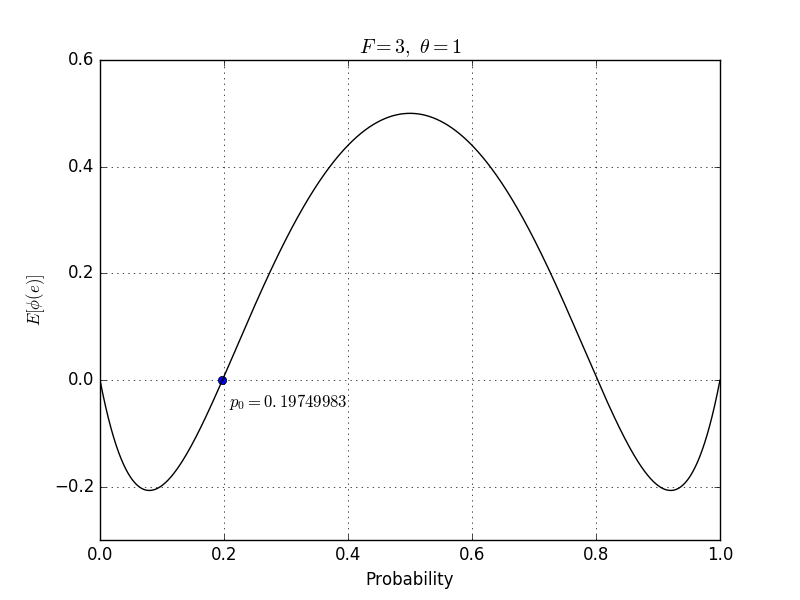
\includegraphics[width=\textwidth]{c:/users/alexander/graphics/F3T1weight.PNG}
  \end{minipage}
  \begin{minipage}[h]{0.45\textwidth}
    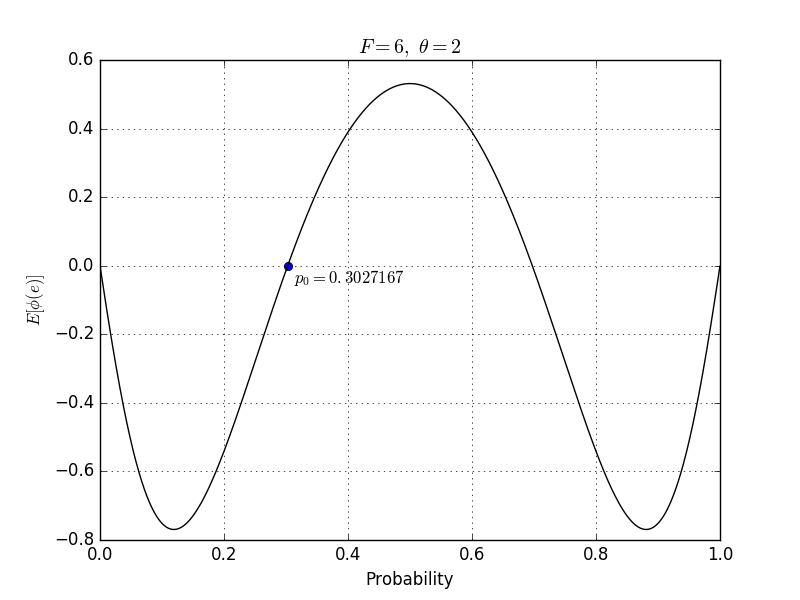
\includegraphics[width=\textwidth]{c:/users/alexander/graphics/F6T2weight.PNG}
  \end{minipage}
    \centering
  \begin{minipage}[h]{0.45\textwidth}
    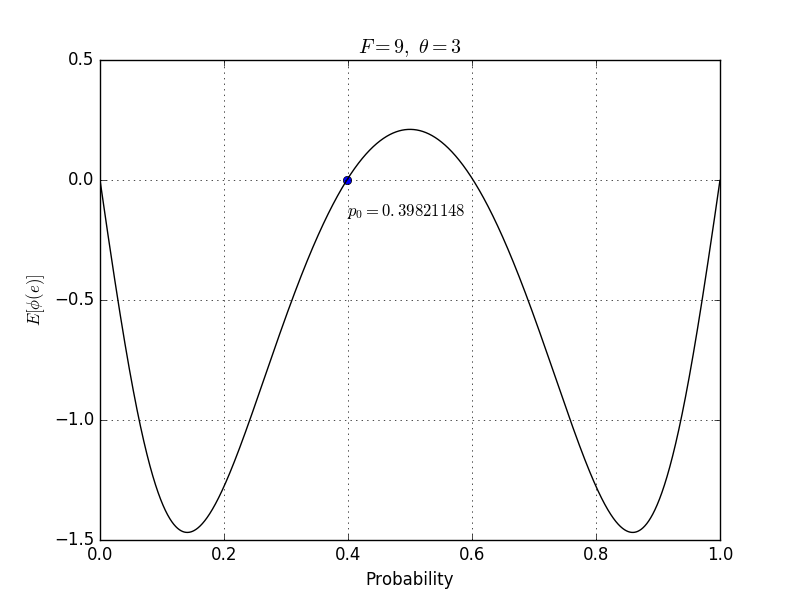
\includegraphics[width=\textwidth]{c:/users/alexander/graphics/F9T3weight.PNG}
  \end{minipage}
  \begin{minipage}[h]{0.45\textwidth}
    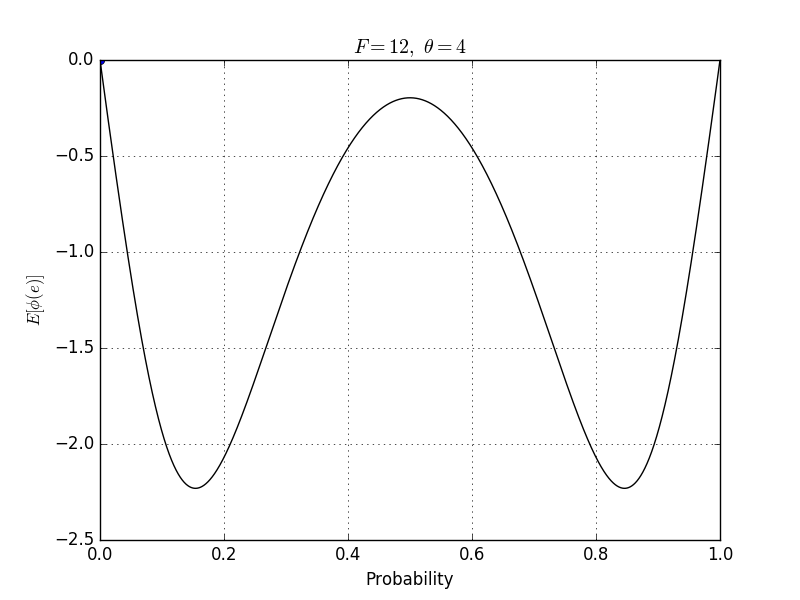
\includegraphics[width=\textwidth]{c:/users/alexander/graphics/F12T4weight.PNG}
  \end{minipage}
  \caption{Fixation cannot be derived for $F=12, \theta = 4$}
\end{figure}

\clearpage

\section{Simulation on the Torus}

Numerical computer simulations are definitely an important complementary method to a deeper understanding of spin systems such as the vectorial Deffuant model. Nonetheless, numerical simulations have have to be interpreted with restraint.\\
Firstly, we simulate a discrete counterpart to the model defined above. The graph, we here use a $100\times 100$ torus, is necessarily finite and the process is a discrete time Markov chain approximated with the Metropolis algorithm. \\
Secondly, stochastic spatial simulations are generally difficult to interpret, especially if they have a number absorbing states. The number of absorbing states of the vectorial Deffuant model grows exponentially with the number of features. Simulations of the finite system can thus freeze in a large number of configurations which are not exemplary or symptomatic of the long-term behaviour of the infinite counterpart. \\
\indent The simulations are done using the simulation toolkit RepastJ. RepastJ provides a number a predefined random number generators, an integrated GUI and a framework for time-scheduling simulations programmed in Java.\\   

\textbf{The local algorithm:}\\
The simulation here is done on a grid with coloured squares, where each square is a site and each colour represents a unique configuration. The grid wraps around the edges to form a torus. The number of features $F$ and the threshold $\theta$ are fixed for the entire simulation. The simulation is started from a product measure where each feature of each site is set to $0$ or $1$ with equal probability. We then simulate the process with a local algorithm (Metropolis). At every 'tick' (step of the simulation) a random site \textit{a} is chosen on the torus. A second site \textit{b} is chosen  from \textit{a}'s neighbourhood at random. We use the so-called \textit{von Neumann} neighbourhood to replicate interaction on a $\mathbb{Z}$-lattice. \textit{a} and \textit{b}'s configuration is compared and the features which differ in configuration are stored in a list. If this list is not greater than the fixed threshold, a feature from the list is chosen at random and the configuration of this feature is set equal for \textit{a} and \textit{b}. Whether \textit{a} or \textit{b} has to change her configuration is decided randomly with equal probability.\\
The interaction defined for the dissociating vec. Deffuant model depends more strongly on the current configurations of \textit{a} and \textit{b}. The code thus consists of several if-statements to simulate the correct flip rates.\\
If \textit{a} and \textit{b} already have the same configuration or they are \textit{incompatible} (number of differing features exceeds threshold), another site is chosen at random and the algorithm is repeated. Up 10000 repetitions are attempted within one 'tick' until a successful interaction is achieved, i.e. until the configuration of some site changes. \\
\newline
The simulation runs at a good speed until it is near an absorbing state, because many sites have to be sampled to find a pair of neighbours who differ and are compatible. This is generally a weakness of local Metropolis algorithms. \\
A so-called sweep, corresponding on average to one evolution of the Markov chain, is completed when on average each site has been sampled. \\
After every 10000 ticks (a fairly substantial amount of interactions) the GUI is updated, such that the colours indicate the current configuration at each site, and a range of data is collected and printed by the program. This data includes:
\begin{itemize}
\item \textbf{Average region size:} A region consists of contiguous sites which all have the same configuration. The program analyses how many sites a region consists of on average.
\item \textbf{Average zone size:}  A zone consists of contiguous sites which are all compatible. The program analyses how many sites a zone consists of on average.
\item \textbf{Number of disagreements:} The number of neighbour pairs which differ in more than $\theta$ features. In other words, this is the number of blocked edges.
\end{itemize}

We simulate the vec. Deff. model for $F=3$ and $F=4$ varying the threshold parameter respectively. The dissociating vec. Deff. model is simulated by additionally varying the $\kappa$ value. An immediate observation for the standard vec. Deff. model was that none of the simulations froze easily. All simulations were stopped at 10 million (for F=3) or 100 million (for F=4) ticks before they had reached an absorbing state. And because of large output intervals (10K for F=3, 100K for F=4) the behaviour of simulations for one set of parameters (e.g. 10 simulations for $F=3$,$\theta=1$) was very consistent. Hence, the the problem that simulations can freeze in atypical configurations did not pose a problem for the standard model. Data was collected and a Monte Carlo average of 10 simulations for each set of parameters was taken. This is by no means a good or accurate Monte Carlo simulation and we do not attempt to make quantitative conclusions about the system. These simulations only serve as an insight to the general behaviour of the system and as an outlook for further research potential.

\subsection{Analyses of Simulation Data }
\subsubsection{Vectorial Deffuant Model, F=3 and F=4}

The simulation data and GUI graphics are depicted below. Figure 14 and 15 show how the simulation evolves from a uniform distribution of configurations to patches of single configurations. In Figure 15 a region is a single colour patch, whereas a zone can consist of several coloured patches where adjacent patches do not differ in more than one feature. The evolution of the number of disagreements, the average zone sizes and the average region sizes in time (ticks) are plotted in Fig. 16, 17 and 18 respectively.

\begin{figure}[h]
  \centering
  \begin{minipage}[b]{0.4\textwidth}
    
\includegraphics[width=\textwidth]{c:/users/alexander/graphics/vDF3T1init.PNG}
    \caption{Initial configuration: F=3, $\theta=1$, $100\times 100$ torus.}
  \end{minipage}
  \hfill
  \begin{minipage}[b]{0.4\textwidth}
    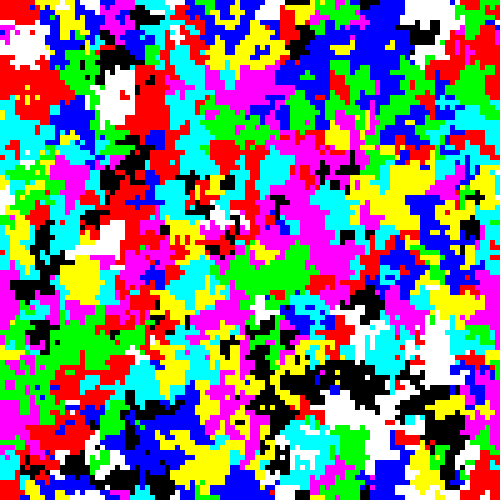
\includegraphics[width=\textwidth]{c:/users/alexander/graphics/vDF3theta1.PNG}
    \caption{The simulation in Fig. 13 after 100 million ticks.}
  \end{minipage}
\end{figure}

\begin{figure}[h]
  \centering
  \begin{minipage}[b]{0.45\textwidth}
    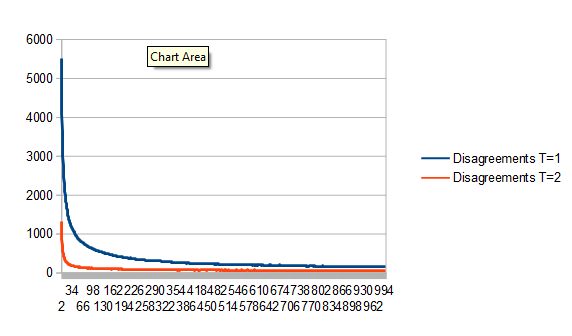
\includegraphics[width=\textwidth]{c:/users/alexander/graphics/F3disagreements.PNG}
  \end{minipage}
  \begin{minipage}[b]{0.45\textwidth}
    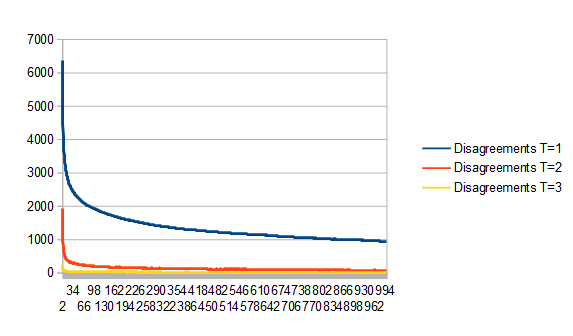
\includegraphics[width=\textwidth]{c:/users/alexander/graphics/F4disagreements.PNG}
  \end{minipage}
  \caption{Disagreements: F=3 (left), F=4 (right) and different $\theta$(T).}
\end{figure}

\clearpage

\begin{figure}[h]
  \centering
  \begin{minipage}[b]{0.45\textwidth}
    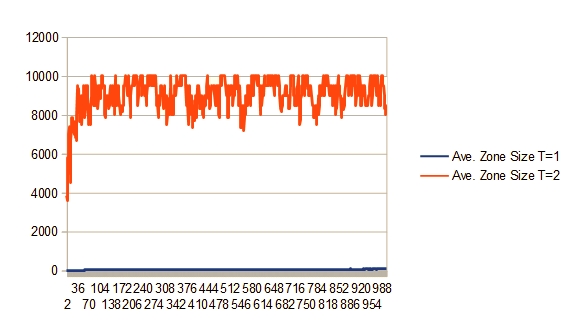
\includegraphics[width=\textwidth]{c:/users/alexander/graphics/F3zones.PNG}
  \end{minipage}
  \begin{minipage}[b]{0.45\textwidth}
    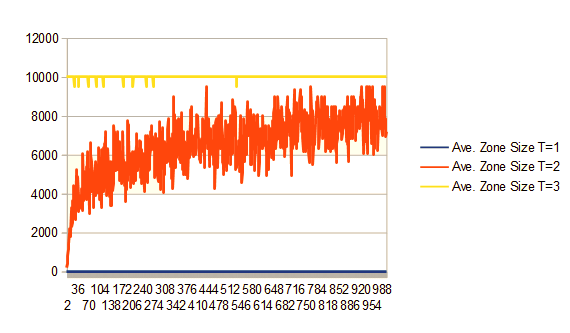
\includegraphics[width=\textwidth]{c:/users/alexander/graphics/F4zones.PNG}
  \end{minipage}
  \caption{Average Zone Size: F=3 (left), F=4 (right) and different $\theta$(T).}
\end{figure}

\begin{figure}[h]
  \centering
  \begin{minipage}[b]{0.45\textwidth}
    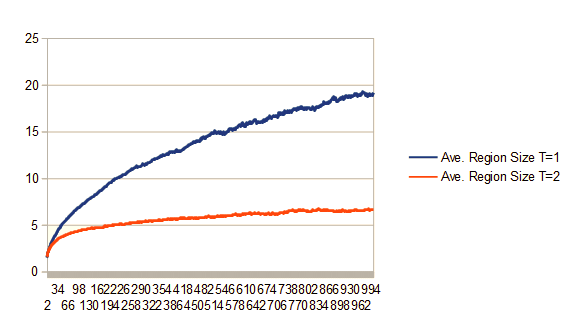
\includegraphics[width=\textwidth]{c:/users/alexander/graphics/F3regions.PNG}
  \end{minipage}
  \begin{minipage}[b]{0.45\textwidth}
    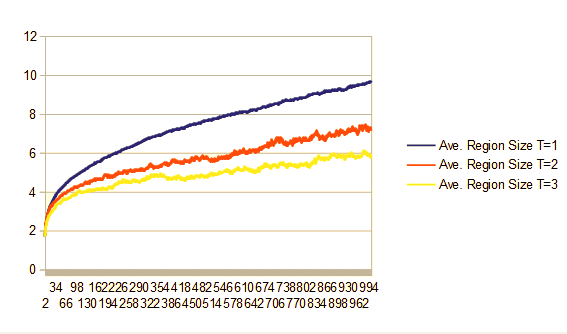
\includegraphics[width=\textwidth]{c:/users/alexander/graphics/F4regions.PNG}
  \end{minipage}
  \caption{Average Region Size: F=3 (left), F=4 (right) and different $\theta$(T)}
\end{figure}

The number of disagreements is lower for higher thresholds and decreases as the system evolves. This not surprising. \\
There seems to be a stark difference in the stability of zones when the threshold is varied. For $\theta=1$ and $F=3$ the average zone size only gradually increases from about 10 to 70 sites. For $\theta=1$ and $F=4$ it gradually increases from 2 to 12 sites. The ave. zone size shows strong fluctuation for an intermediate threshold. This is due to the fragmentation of zones. Even though larger zones are stable smaller zones are created and destroyed continuously. A larger sample size would most probably produce smoother curves. When $\theta$ is close to $F$ ($\theta = F-1$ here) the entire torus is a single zone for most of the simulation. \\
The average region size seems to evolve counter-intuitively. A lower threshold produces larger regions. For higher thresholds, there is a higher fluctuation of configuration and regions remain in a more fragmented state.  
The dissociating vec. Deff. model with a large threshold could, for certain values of $\kappa$, display larger average region sizes and reduced fluctuation. In following subsection we do the same simulations with varying values for $\kappa$.

\subsubsection{Dissociating Vec. Deff. Model, F=3 and F=4}

When simulating the dissociating vectorial Deffuant model we see for $\kappa >1$ an increased growth of the average region sizes. However, the diss. vec. Deff. model does not induce stability of all regions. Only regions of trivial configuration 0 and 1 grow exponentially. Furthermore, a large $\kappa$ will cause the system to freeze and the stability of average zone size is compromised. \\
\begin{figure}[h]
  \centering
  \begin{minipage}[h]{0.45\textwidth}
    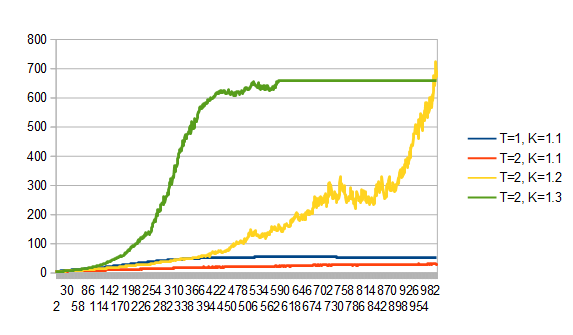
\includegraphics[width=\textwidth]{c:/users/alexander/graphics/diss3RegionSize.PNG}
  \end{minipage}
  \begin{minipage}[h]{0.45\textwidth}
    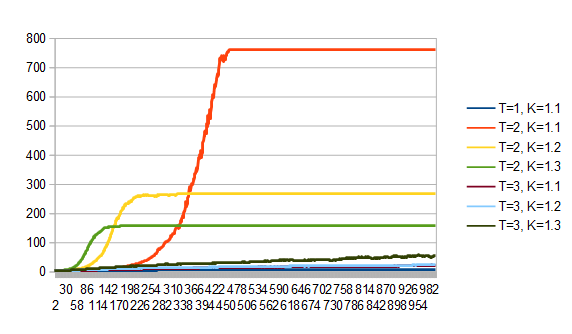
\includegraphics[width=\textwidth]{c:/users/alexander/graphics/diss4RegionSize.PNG}
  \end{minipage}
  \caption{Average Region Size: F=3 (left), F=4 (right) and different $\theta$(denoted T),$\kappa$ (K).}
\end{figure} 
 
\begin{figure}[h]
  \centering
  \begin{minipage}[h]{0.45\textwidth}
    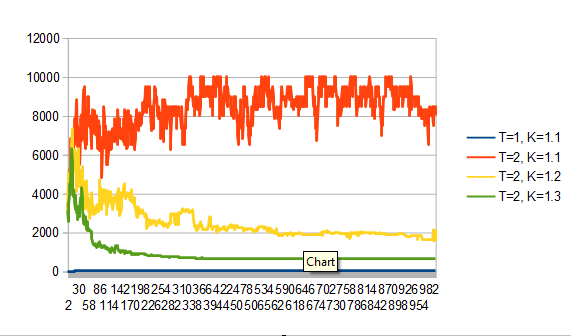
\includegraphics[width=\textwidth]{c:/users/alexander/graphics/diss3ZoneSize.PNG}
  \end{minipage}
  \begin{minipage}[h]{0.45\textwidth}
    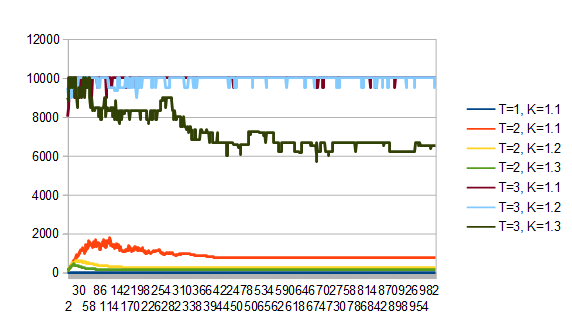
\includegraphics[width=\textwidth]{c:/users/alexander/graphics/diss4ZoneSize.PNG}
  \end{minipage}
  \caption{Average Zone Size: F=3 (left), F=4 (right) and different $\theta$(denoted T),$\kappa$ (K).}
\end{figure}
In Figure 19. for $F=4, \theta =2$, $\kappa =1.3$ and $F=3, \theta =2, \kappa =1.3$, we see a sharp increase in the average region size for large $\kappa$ initially, the growth rate then becomes slower and eventually becomes constantly 0. This is due to simulations freezing, i.e. once the ave. region size is constant all sample simulations have frozen. Neither a decrease in the growth rate nor the existence of an equilibrium for the ave. region size must be symptomatic of the infinite system. We do, however, see that a larger average region size can be achieved using a small $\kappa >1 $ and hereby inducing a more gradual growth. In the diagram on the right of Figure 19. (F=4) we still see thresholds 1 and 2 promoting a higher region growth than threshold 3. The parameter $\theta = 2, \kappa =1.1$ may be the best combination for achieving large regions, however, it is not certain if the average region size for the combinations with $\theta =3$ will steadily continue to grow -- $\theta =3, \kappa =1.1$ may eventually achieve the largest region sizes eventually.
Figure 20. depicts the evolution of average zone sizes. We see a strong loss of stability in average zone sizes for large $\kappa >1$. Especially low thresholds coupled with a large $\kappa$ cause the ave. zone size to deteriorate. Only in the case that $F=4, \theta=3$ and $\kappa=1.1,1.2$ are the zone sizes large and stable.\\

A high threshold and a value for $\kappa$ near 1.1 may well be most suitable applying the model to social phenomena. We discuss the linguistic interpretation in more detail in the next and final section.  

\subsection{Implications for Simulating Language Change}

In order to determine which parameter values are reasonable when simulating the northern cities vowel shift, for example, one would have to study empirical data. A simulation of this sort could, with sufficient manipulation, fit the data. It is, however, not our opinion that a simulation can explain a sound change in its entirety. The objective is rather to understand what the core mechanisms behind a sound change are. The behaviour of real language populations should be compared to the behaviour of simulations. And there a several interesting questions which can be asked:
\begin{itemize}
\item Does a high fluctuation in pronunciation, both synchronically and diachronically, coincide with a readiness in the population to imitate the speech of others who possibly speak very differently?
\item Is it reasonable to assume that a speech community always constitutes on zone, i.e. are all individuals connected through a chain of alliances which allow an exchange of pronunciation traits?
\item How are disagreements distributed in a speech community?
\item How is the implementation of a sound change, i.e. the lexemes undergoing change, perceived in a speech community? Is it fragmented or regular?
\item Does a sudden spread of a new pronunciation lead to a polarization of the speech community? 
\end{itemize} 
Arguably, every model composes a theory in itself. And the central assumptions, homophily and social influence, are of an inductive nature even if they aren't strong assumptions. The dissociating vectorial Deffuant makes a somewhat stronger assumption, an assumption of regularity: individuals will when imitating each others speech tend to adopt pronunciations which make the use of the phoneme more regular. They tend to assume the trivial configuration $0$ and $1$ more readily. How reasonable this assumption is may depend on the speech community in question. In Figure 21. and 22. we compare a simulation of the vectorial Deffuant model ($F=8, \theta=6$) and the dissociating vectorial Deffuant model ($F=8, \theta=6, \kappa =1.1$) on the $100\times 100$ torus. The figure depicts both simulations after 3 million ticks, where the entire torus comprises a single zone in both simulations. The dissociating vec. Deff. model shows a very natural topology of two groups with regular pronunciation patterns (black and white regions) connected by individuals with intermediate configurations. Hence, the regularity assumption produces a speech community dynamic which we would expect. The standard vec. Deff. model in contrast shows a more fragmented speech community. 
 
\begin{figure}[h]
  \centering
  \begin{minipage}[h]{0.4\textwidth}
    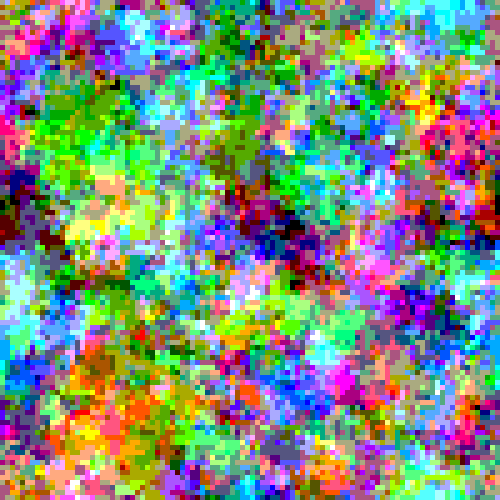
\includegraphics[width=\textwidth]{c:/users/alexander/graphics/vD8-63m.PNG}
    \caption{F=8, $\theta=6$, $\kappa =1.0$, 3m ticks.}
  \end{minipage}
  \hfill
  \begin{minipage}[h]{0.4\textwidth}
    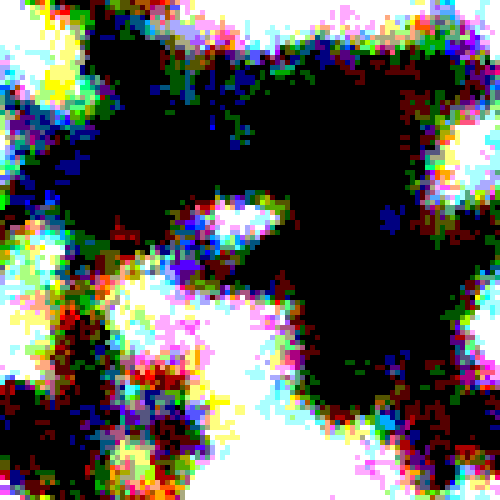
\includegraphics[width=\textwidth]{c:/users/alexander/graphics/dissVD8-63m.PNG}
    \caption{F=8, $\theta=6$, $\kappa =1.1$, 3m ticks.}
  \end{minipage}
\end{figure}

Where a great deal of improvement and experimentation can be made, is in the initial configuration of the system. Any hypothetical distribution or a distribution motivated by empirical data can be used to start the system. Here we only considered the system started from a product measure with positive type densities -- in the simulations this density was always a half. The social network, the graph of the system, can also be adjusted to reflect specific social topologies. Stauffer and Schulze noted in \cite{Schulze} that there is a need for a simulation model which displays smaller speech communities who are resilient to adapting to more populous standards. Both the dissociating and the standard vec. Deff. model can display smaller stable zones and this characteristic can be sharpened by manipulating the connectivity of the network.

The significance of this research is that it illuminates the complexity of social interaction of which we, at first, believed to understand all consequences. However, convergent interaction rules can lead to a polarization of the community. And a much larger community can be in fact involved in the process of a vowel shift than the community which finally adopts a new pronunciation standard. 


\clearpage

\section{Appendix A}

\subsection{Duality for (biased) Voter Model d=1}
The (biased) Voter Model on $\mathbb{Z}$ is a continuous time Feller process $\rho_t:\mathbb{Z} \longrightarrow \{ 0,1 \}$ formally given by: the state at $x \in \mathbb{Z}$ flips  
\begin{equation}
\begin{split}
& 0 \longrightarrow 1 \text{ at rate } \frac{1}{2}\vert\{ y \sim x: \rho(y)=1 \} \vert \text{ and}\\ 
& 1 \longrightarrow 0 \text{ at rate } \kappa\frac{1}{2}\vert\{ y \sim x: \rho(y)=0 \} \vert,
\end{split}
\end{equation} 
where $\kappa \geq 1$ and $\kappa = 1$ gives the standard voter model. \
We construct the graphical representation as in Section 2.4. from a collection of independent rate 1 Poisson processes $(N_n^{x,y}(t): t \geq 0)$, with arrival times $(T^{x,y}(n): n \geq 1)$ and a collection of independent Bernoulli random variables $(B^{x,y}_n: n \geq 1)$ such that $P(B^{x,y}_n=+1 \vert \rho_{T^{x,y}(n)-}(x)=1,\rho_{T^{x,y}(n)-}(y)=0 )= \frac{\kappa}{\kappa+1}$ and $P(B^{x,y}_n=-1 \vert \rho_{T^{x,y}(n)-}(x)=1,\rho_{T^{x,y}(n)-}(y)=0 )= \frac{1}{\kappa+1}$ and so forth. \\
We say that there exists a dual path from $(x,t)$ to $(z,t-s)$ for $0 \leq s \leq t$, if there is a path from $(z,t-s)$ to $(x,t)$, and we define the dual process starting at $(A,t)$ for a set $A \subset \mathbb{Z}$ by setting
$$\hat{\rho}_s^{(A,t)} = \{ z \in \mathbb{Z}: \text{ there is dual path from } (x,t) \text{ to } (z,t-s) \text{ for an } x \in A\}$$
for any $0 \leq s \leq t$. It is convenient to assume that the Poisson processes are also defined for negative times, so that the dual process is naturally defined for all $s \geq 0$. \\
For any fixed realization of the graphical representation for each $x \in \mathbb{Z}$ and any $s<t$ there is a unique $z \in \mathbb{Z}$ such that there is a dual path from $(x,t)$ to $(z,s)$.
The dual process is \textit{additive}, i.e. $\hat{\rho}_s^{(A \cup B,t)}= \hat{\rho}_s^{(A,t)} \cup \hat{\rho}_s^{(B,t)} \: A,B \subset \mathbb{Z}$. \
In particular the dual process from two sites $x$ and $y$ amounts to running two individual dual processes, $\hat{\rho}_s^{(x,t)}$ and $\hat{\rho}_s^{(y,t)}$, independently until their $\mathbb{Z}$ coordinates are the same, at which point they coalesce. After coalescing the two processes move together. For $p= \frac{1}{2}$ the process $\hat{\rho}_s^{(x,t)}$ performs a continuous time random walk on $\mathbb{Z}$. This implies a duality between the standard voter model and coalescing random walks. 
\clearpage


\begin{thebibliography}{5}

\bibitem{Axelrod} R. Axelrod, \emph{The Dissemination of Culture}, Journal of Conflict Resolution 2 (41), 203-226 (1997)

\bibitem{Griffeath81} M. Bramson and D. Griffeath, \emph{On the Williams-Bjerknes Tumour Growth Model I}, Ann. Probab. 9 (2), 173-185 (1981)

\bibitem{Griffeath89} M. Bramson and D. Griffeath, \emph{Flux and Fixation in cyclic particle systems. }, Ann. Probab. 17 (1), 26-45 (1989)

\bibitem{Castellano} C. Castellano and S. Fortunato and V. Loreto, \emph{Statistical physics of social dynamics}, Reviews of Modern Physics 81, 591-646 (2009)

\bibitem{Chen} M. Chen and W. Wang, \emph{Sound Change: Actuation and Implementation}, Language 51, 255-281 (1975)

\bibitem{Cox} J.T. Cox and D. Griffeath, \emph{Occupation time limit theorems for the voter model.}, Ann. Probab. 11, 876-893 (1983)

\bibitem{Deffuant et al.} G. Deffuant, D. Neau, F.Amblard and G. Weisbuch, \emph{Mixing beliefs among interacting agents.}, Adv. Compl. Sys. 3, 87-98 (2000)

\bibitem{Harris} T.E. Harris, \emph{Nearest-neighbor Markov interaction processes on multidimensionsional lattices}, Advances in Math. 9, 66-89 (1972)

\bibitem{Labov} W. Labov, \emph{Resolving the Neogrammarian Controversy}, Language 57 (2), 267-308 (1981)

\bibitem{AxelrodRevised} N. Lanchier, \emph{The Axelrod Model for the Dissemination of Culture Revised}, Ann. Appl. Probab. 22 (2), 860-880 (2012)

\bibitem{FixAxel} N. Lanchier and S. Scarlatos, \emph{Fixation in the One-dimensional Axelrod Model}, Ann. Appl. Probab. 23 (6), 2538-2559 (2013)

\bibitem{ClustCoex} N. Lanchier and S. Scarlatos, \emph{Clustering and coexistence in the one-dimensional vectorial Deffuant model}, Lat. Am. J. Probab. Math. Stat. 11 (2), 541-564 (2014)

\bibitem{FluxvsFix} N. Lanchier and S. Scarlatos, \emph{Fluctuation versus fixation in the one-dimensional constrained voter model}, ArXiv Mathematics e-prints (2014)

\bibitem{Liggett} T.M. Liggett, \emph{Continuous Time Markov Processes}, AMS. Graduate Studies in Mathematics v. 113 (2010)

\bibitem{Schulze} D. Stauffer and C. Schulze, \emph{Microscopic and Macroscopic Simulation of Competition between Languages}, Physics of Life Reviews 2 (2), 86-116 (2005)

\end{thebibliography}

\newpage
\section*{Declaration of originality}
I hereby confirm that I have written the accompanying thesis by myself, without contributions from any sources other than those cited in the text and acknowledgements. This applies also to all graphics, codes and images included in the thesis.
\\[2cm]
\begin{minipage}{0.4\textwidth}
\begin{flushleft}
\rule{5cm}{0.4pt}
Alexander Mendelsohn
\end{flushleft}
\end{minipage}
\hfill
\begin{minipage}{0.4\textwidth}
\begin{flushright}
\rule{5cm}{0.4pt}
Place, Date
\end{flushright}
\end{minipage}

\end{document}
